\section{Dataset}
Dataset is a collection of data that is related to work and is created to fullfill algorithm requirements being in suitabel dataformat.
In object detection dataset is usually an multimedia data like images or videos but it can be other data type,
such as point clouds. \cite{object_detection_review}

Sometimes there is not suitable dataset available for the work. In that case new dataset is needed to be created. Dataset creation is divided in this to the two phase:
data collection and annotation \cite{object_detection_review}.
Data collection



sliding windows method and Haar featurs
It's idea was very simple as using sliding windows for detection, but speed-up techniques was why it was markable in era where computional power was not so great as now adays. Several techniques was used for speeding-up object detection but as taking cascaded detection as one example, it is a technique where with simple calculations is used filtering simpliest windows and then using complicated calculations for complex windows. \cite{object_detection_20years}


\section{Time-Of-Flight cameras}
CHANGE DEPTH IMAGE TO DEPTH MAP
Time-Of-Flight (ToF) cameras usually discribed being affordable, compact sized and low powered option for estimating distance of the scene with high frame rate\cite{TI2019} \cite{indepth}.
The depth measuring of the ToF cameras is based on sending modulated infrared light to the scene and capturing
the reflected light \cite{inproceedings}\cite{tof}\cite{vizta}. Based on information of the reflected light,
distance and amplitude image, also known as gray-scale image, can be formed. Distance image is calculated from phase difference between emitted
and reflected light and amplitude image from reflected signals amplitude for every corresponding pixel location of the scene. \cite{InfineonReal3} \cite{inproceedings}

The basis idea of ToF cameras depth measuring is based following formula

\begin{equation}
    \rho = \frac{c\tau}{2}
\end{equation}

where $\rho$ is a estimated radial distance, $c$ is light speed (~300 000 000 m/s) and $\tau$ is traveled time of the light from
sensor emittor and receiver\cite{tof}.

Image bellow demonstrates the basic idea of ToF camera depth measuring.





ToF cameras has several usefull features compared to RGB or monochome cameras. In addition to cabable
of measuring distance of the scene, ToF cameras are more resilien to enviromental light changes and color differences \cite{vizta}.
Also depth images provides more privacy as the not has not the same level of detail compared to RGB images \cite{vizta}.


ToF cameras depth images can be affected by several factors that might cause error like artifacts or missing depth information.
These factors are usually distance of the scene points, surface orientation, low reflective objects like dark objects and strong specular reflectors
like mirrors or some metallic surfaces. \cite{indepth} Next previous factors are descriped in more detail.
The effective range of ToF camera is usually within a few meters \cite{?}. Because the measurement is based on phase difference between emitted and reflected light,
the maximum measurable distance depends on the modulation frequency of the light source. The maximum measurable distance can be defined as

\begin{equation}
    d_{amb} = \frac{c}{2f}
\end{equation}

where $d_{amb}$ is the ambiguity distance and $f$ is the modulation frequency of the light source \cite{Time-of-Flight Camera – An Introduction}.
Because phase wraps around every $2\pi$, the distace alliacing will occur if the distance of the scene point is greater than $d_{amb}$ \cite{Time-of-Flight Camera – An Introduction}.
Measurement distance can be extended for example increasing modulation frequency when also accuracy redusing or using other
techniques like multi-frequency techique \cite{Time-of-Flight Camera – An Introduction}.

Different surfaces can affect depth images multiple way. Brightness of the surface can intefere with
emitted infrared light which may give measure error if surface is overly bright \cite{Time-of-Flight Camera – An Introduction}.
Also dark surfaces can cause error because of low reflectivity. For example reflectivity of black denim cloth is about 10 \%.
Because the dark surface absobing mayor part of the emitted light, it may cause holes in depth image. \cite{Time-of-Flight Camera – An Introduction} \cite{indepth}
Strong specular reflectors surfaces can cause  misdirecting the emitted signal away from sensor,
causing it to perceive the reflected scene as the target, or by returning excessive light, which lead to system saturation \cite{TI2019}.
Orientation of surface can cause error because high indicent angle of reflected light could be too weak to be detected \cite{indepth}.

In this work we not observe some of the previous error sources like from mirrors that can show falsely reflected scene as target.
Instead we try to introduce some methods that removes holes and artifacts from resulting depth images.



Physical idea of ToF-sensors are similar compared to Lidar (Light detection and ranging) scanners. The difference
between them is that ToF-sensors scanning scene subsequentlu, while Lidar scanners scans the scene .



Most typical illuminators of ToF sensors are LED (Light Emitting Diode),
Edge-Emitting Laser and VCSEL (Vertical-cavity surface-emitting laser) \cite{TI2019}.

3D ToF cameras uses own illumination source, which is usually modulated infrared light. Based on reflected infrared light,
depth and amplitude images can be formed. Depth image is computed by measuring phase shift between emitted and reflected light.
Amplitude image is estimated by reflected signals amblitude. \cite{inproceedings}





%\section{Flexx2 - 3D Camera}
%REAL3™ 3D Image Sensor provides depth and amplitude data of the scene.
%Sensor projects a single modulated infrared light source to the scene and
%captures the reflected light.\cite{InfineonReal3} In this recearch used sensor is model IRS2381C which uses VCSEL 
%(Vertical-cavity surface-emitting laser) as illumination driver sending modulated near infraled light with 940nm wavelenght \cite{IRS2381C}. 
%Captured reflected light goes through the lense of the ToF imager. In the ToF imager amplitude and phase difference between emitted
%and reflected light are measured for corresponding pixel of the scene. Measurements from the pixel matrix are sended to
%host controller using analog digital converter. Host controller process data to create 
%depth and amplitude data. \cite{InfineonReal3} \cite{IRS2381C}







can generate depth map of the scene by measuring traveled time of the emitted electo-magnetic
raditation from the sensor and back when it reflects back from the scene surface \cite{tof}\cite{vizta}.

Because the infrared light goes light speed  in air, the estimated radial distance between
sensor and a scene point can be calculated using formula

Because the distance measurement is done based comparing phase difference between emitted and reflected Light
maximum measurable distance can be defined as

% \begin{figure}[!h]
%     \centering
%     \includegraphics[width=0.5\textwidth]{images/tof_camera.png}
%     \caption{ToF camera depth measuring}
%    \label{fig:tof_camera}
% \end{figure}



@article{voxelnet,
  author={Zhou, Yin and Tuzel, Oncel},
  booktitle={2018 IEEE/CVF Conference on Computer Vision and Pattern Recognition}, 
  title={VoxelNet: End-to-End Learning for Point Cloud Based 3D Object Detection}, 
  year={2018},
  volume={},
  number={},
  pages={4490-4499},
  keywords={Three-dimensional displays;Laser radar;Feature extraction;Shape;Proposals;Encoding},
  doi={10.1109/CVPR.2018.00472},
  }

  @manual{TI2019,
    title = {Introduction to Time-of-Flight Long Range Proximity and Distance Sensor System Design (Rev. B)},
    author = {Texas Instruments},
    year = {2019},
    address = {Dallas, Texas},
    url = {https://www.ti.com/lit/pdf/sbau305}
}

@article{indepth,
author = {Zhang, Yunfan and Scargill, Tim and Vaishnav, Ashutosh and Premsankar, Gopika and Di Francesco, Mario and Gorlatova, Maria},
title = {InDepth: Real-time Depth Inpainting for Mobile Augmented Reality},
year = {2022},
issue_date = {March 2022},
publisher = {Association for Computing Machinery},
address = {New York, NY, USA},
volume = {6},
number = {1},
url = {https://doi.org/10.1145/3517260},
doi = {10.1145/3517260},
abstract = {Mobile Augmented Reality (AR) demands realistic rendering of virtual content that seamlessly blends into the physical environment. For this reason, AR headsets and recent smartphones are increasingly equipped with Time-of-Flight (ToF) cameras to acquire depth maps of a scene in real-time. ToF cameras are cheap and fast, however, they suffer from several issues that affect the quality of depth data, ultimately hampering their use for mobile AR. Among them, scale errors of virtual objects - appearing much bigger or smaller than what they should be - are particularly noticeable and unpleasant. This article specifically addresses these challenges by proposing InDepth, a real-time depth inpainting system based on edge computing. InDepth employs a novel deep neural network (DNN) architecture to improve the accuracy of depth maps obtained from ToF cameras. The DNN fills holes and corrects artifacts in the depth maps with high accuracy and eight times lower inference time than the state of the art. An extensive performance evaluation in real settings shows that InDepth reduces the mean absolute error by a factor of four with respect to ARCore DepthLab. Finally, a user study reveals that InDepth is effective in rendering correctly-scaled virtual objects, outperforming DepthLab.},
journal = {Proc. ACM Interact. Mob. Wearable Ubiquitous Technol.},
month = {mar},
articleno = {37},
numpages = {25},
keywords = {Augmented reality, depth inpainting, depth sensing, edge computing, user experience}
}


@techreport{IRS2381C,
    author = {Infineon Technologies AG},
    title = {Product brief REAL3™ image sensor IRS2381C 3D Time-of-Flight single-chip},
    year = {2019},
    address = {Munich, Germany},
    urldate   = {2024-15-2},
    url = {https://www.mouser.com/pdfDocs/Infineon-REAL3_image_sensor_IRS2381C-PB-v01_00-EN.pdf},
    langid  = {english}
}

@misc{InfineonReal3,
    author = {Infineon Technologies AG},
    title = {ToF 3D image sensors},
    url = {http://www.infineon.com/real3},
    urldate   = {2024-15-2},
    langid  = {english}
}

@inproceedings{inproceedings,
author = {Oprisescu, Serban and Falie, Dragos and Ciuc, Mihai and Buzuloiu, Vasile},
year = {2007},
month = {08},
pages = {1 - 4},
title = {Measurements with ToE Cameras and Their Necessary Corrections},
volume = {1},
isbn = {1-4244-0969-1},
journal = {ISSCS 2007 - International Symposium on Signals, Circuits and Systems, Proceedings},
doi = {10.1109/ISSCS.2007.4292691}
}


@book{tof,
publisher = {Springer New York},
series = {SpringerBriefs in Electrical and Computer Engineering},
year = {2012},
title = {Time-of-Flight Cameras and Microsoft Kinect™},
abstract = {Time-of-Flight Cameras and Microsoft Kinect™ closely examines the technology and general characteristics of time-of-flight range cameras, and outlines the best methods for maximizing the data captured by these devices. This book also analyzes the calibration issues that some end-users may face when using these type of cameras for research, and suggests methods for improving the real-time 3D reconstruction of dynamic and static scenes. Time-of-Flight Cameras and Microsoft Kinect™ is intended for researchers and advanced-level students as a reference guide for time-of-flight cameras. Practitioners working in a related field will also find the book valuable.},
author = {Dal Mutto, Carlo. and Zanuttigh, Pietro. and Cortelazzo, Guido M.},
address = {New York, NY},
edition = {1st ed. 2012.},
isbn = {1-280-79507-7},
keywords = {Signal processing},
language = {eng},
}


\begin{table}[ht]
    \begin{tabular}{|l|r|r|r|r|}
    \hline
    Model & Precision\textsubscript{IoU:50} & Recall\textsubscript{IoU:50} & F1\textsubscript{IoU:50} & AP\textsubscript{IoU:50-95} \\
    \hline
    s500 & 0.482 & 0.924 & 0.634 & - \\
    s1000 & 0.740 & 0.901 & 0.813 & - \\
    s1500 & 0.787 & 0.892 & 0.836 & - \\
    s2000 & 0.854 & 0.883 & 0.869 & - \\
    s2500 & 0.847 & 0.848 & 0.848 & - \\
    \hline
    r200 & 0.364 & 0.905 & 0.519 & -\\
    r200s500 & 0.748 & 0.845 & 0.793 & -\\
    r200s1000 & 0.790 & 0.881 & 0.833 & - \\
    r200s1500 & 0.847 & 0.882 & 0.864 & - \\
    r200s2000 & 0.840 & 0.913 & 0.875 & - \\
    r200s2500 & 0.886 & 0.887 & 0.887 & - \\
    \hline
    r400 & 0.529 & 0.916 & 0.671 & - \\
    r400s500 & 0.781 & 0.879 & 0.827 & - \\
    r400s1000 & 0.821 & \textbf{0.930} & 0.872 & -\\
    r400s1500 & 0.867 & 0.906 & 0.886 & - \\
    r400s2000 & 0.880 & 0.897 & 0.888 & - \\
    r400s2500 & 0.856 & 0.922 & 0.888 & - \\
    \hline
    r568 & 0.802 & 0.915 & 0.855 & - \\
    r568s500 & 0.883 & 0.885 & 0.884 & - \\
    r568s1000 & 0.855 & 0.892 & 0.873 & - \\
    r568s1500 & 0.869 & 0.889 & 0.879 & - \\
    r568s2000 & 0.893 & 0.895 & 0.894 & - \\
    r568s2500 & \textbf{0.897} & 0.909 & \textbf{0.903} & - \\
    \hline
    \hline
    yolov8n (Base) & 0.877 & 0.657 & 0.751 & - \\
    \hline
    \end{tabular}
    \caption{Comparisons of fine-tuned YOLOv8n models with freezed-layers and the base model} 
    \label{tab:results}
    \end{table}
    

    \begin{table}[!h]
        \begin{tabular}{c|c|c}
        Theme & Synthetic image generation method &  Synthetic image generation tool   \\
        Aerial object detection  & finetuned diffusion-based synthetic image generation & Stable diffusion and LORA finetuning\\
        In-car cabin monitoring & 3D simulation & Blender and other tools for creating 3D-models\\
        Milk package detection in refrigerator & Blending objects into real photos & SegmentAnything was used extract objects from existing datasets for blending into new background\\
        Traffic vehicles detection and classification in urban application & diffusion-based synthetic image generation & Kandinsky 2.2\\
        Industrial object detection &  GAN models for synthetic image generation & Different \\
        Aerial ship detection& &Blender and\\
        Motorcyclists' helmet violation detection & &\\
        Heavy machinery detection and classification & & \\
        Downstream road detection & CRS-Diff: Controllable Remote Sensing Image Generation with Diffusion Model & \\ 
    
        https://arxiv.org/html/2403.11614v4
        Underwater Mine-like Object Detection & images generated via the Diffusion Mode & \\ 
    
        https://arxiv.org/abs/2410.12953
    
        " GANs to generate realistic synthetic data not only increases the diversity and quantity of training data but also improves the adaptability of the object detection model to the complexities and variations in real industrial scenarios" 
        \end{tabular}
        \end{table}

        Training batch size & How many images are taken in training at the same time. Speeding up training but make training using more VRAM. Increasing batch size can make it model slightly better or worse, but value between 1-4 should be fine. \\
    \hline
    Epoch & define sets of learning. With option Save every N epoch it saves LoRA model of current state. Affects total learning steps.\\
    \hline
    LR (learning rate) Scheduler & controls learning rate during the training. Basic schedulers are constant, cosine and linear scheduler. Constant scheduler keeps learning rate same and linear shculer decreases learning rate linearly toward 0 during the training. Cosine scheduler degreases learning rate toward 0 following wave of cosine curve. \\
    \hline
    Learning rate warmup (only for constant scheduler)& increases learning rate linearly from 0 to given learning rate within given prosent value. Percent value is taken from total training steps. \\
    \hline
    Optimizer & Set algorithm to update neural net weight and trying to reduce error during training . There is many different potimizers but usually used are AdamW, AdamW8bit and Adafactor. AdamW is a variant of the Adam optimizer that has weight decay regularization and Adaw8bit is version that uses less VRAM and has less accuracy than AdamW. Adafactor will ignora learning rate settings as it adjust learning rate while training.\\
    \hline
    Learning rate Unet &  Sets the learning rate for U-Net ! if set it takes precedence over learning rate \\
    \hline
    Learning rate TE (text encoder) & Determines the sensitivity to captions. As it affects whole Unet, TE learning rate is usually about half from Unet learning rate ! if set it takes precedence over learning rate \\
    \hline
    Max resolution & Set the border of the used resolution of images. Images that width or height is over setted max resolution will be scaled down to setted resolution\\
    \hline
    Enable buckets & Buckets are containers for different image sizes as in training different sized images can't be trained as the same time. If there is only same sized images Bucket are not nesessary.  \\
    \hline
    Minimum/Maximum bucket resolution &  Set the border of the buckets resolution\\
    \hline
    Minimum/Maximum bucket resolution & - \\
    \hline
    Minimum/Maximum bucket resolution & - \\
    \hline
    Minimum/Maximum bucket resolution & - \\
    \hline


    
Custom LoRA model creation needs robust collection of images from wanted topic [?]. As we want to test can it be created people detection model for NIR images inside elevetor, it is needed differented images around that topic. For training LoRA model there was used 31 cherry-picked images from the dataset. The LoRA training collection was crated by taking a few images from different recordings. This way collection was robust for training as it includes for example images with different background, lighting, people, objects and positioning. 

%In  This makes latent space $z$ 48-times smaller than original image $x$.

%\cite{rombach2022highresolutionimagesynthesislatent}
%One key problem with diffusion models is that training is very slow and heavy if it is used high-resolution images. There is different approacess like training text-to-image model on lower resolution images and use other neural network to upsample and sharpening images.[?] In latent diffusion model this is solved by compressing and reconstruct images using variational autoencoder (VAE). VAE is CNN that is trained to encode images to lower dimensional latent space and decode latent space back to images \cite{esser2021tamingtransformershighresolutionimage}. A Latent space is compressed representation of data that has information of features while discarding irrelevant details of the data [https://arxiv.org/abs/1312.6114]. In first step of training the latent diffusion model, the input image $x$ is encoded with encoder $\mathcal{E}$ to latent space $z$. This can be represented as

%\begin{equation}
%z=\mathcal{E}(x) \tag{2}
%\end{equation}
%where $x \in \mathbb{R}^{H \times W \times 3} $ reprecenting three channeled RGB image with height $H$ and width $W$ and $z \in \mathbb{R}^{H/8 \times W/8 \times 4} $ is .This makes latent space $z$ 48-times smaller than original image $x$.
%The encoder $\mathcal{E}$ is variational autoencoder (VAE) that is CNN with single self-attention mechanism which is trained image dataset. 

%\begin{equation}
%L_{L D M}:=\mathbb{E}_{\mathcal{E}(x), \epsilon \sim \mathcal{N}(0,1), t}\left[\left\|\epsilon-\epsilon_{\theta}\left(z_{t}, t\right)\right\|_{2}^{2}\right] \tag{2}
%\end{equation}


%To create synthetic images that has wanted features as images taken from NIR-sensor, it is needed to create LoRA model to fine-tune main model to do so. In this section is introduced how final LoRA model was created and what parameters were used in training. 




%In this work two different trained LoRA models were used later for generatin synthetic images. First one was  trained without annotations and second one was trained with annotations. Tämä toteutettiin siksi koska haluttiin nähdä kuinka annotointi vaikuttaa synteettisten kuvien generoinnissa.
 


As SDXL has preverences to use certain resolutions to image generation it is good to try get our training images scaled close to following resolotions
%[https://platform.stability.ai/docs/api-reference#tag/SDXL-and-SD1.6/operation/textToImage] [https://stability.ai/sdxl-aws-documentation]


For LoRA training preprosessing, sensor images are scaled within that resolution range. For upscaling images open source tool Upscayl is used. Also it scale images it provides super-resolution methdos like real-ersgan and ultrasharp. Because SDXL is base model is trained by using high resolution images it was tought that it would be good use super-resolution methods to get rid of blurriness of normally scaled images and so emphasizes patterns of the orginal image. Below there is two images where other is resized using only Python Imaging Library (PIL) and other is scaled using Upscayl with ultrasharp model for super-resolution:

-- Normal (left) and super-resolution (right) scaled image -- 

As seen from the figure, image where PIL is only used for scaling is blurry


Every selected image was labeled as discraiping what is happening in the image. 
 

KIRJOITA TAULUKKO JOSSA ON TERMI, KUVAUS, OLETUS ARVO JA KÄYTETTY ARVO sekä MIKSI KÄYTETTY ARVO ON VALITTU


In this work for Lora training is used Kohya's GUI (aka kohya ss) which provides user friendly interface to train lora models. 
It also provides tools for model conversion, training textual inversion, Checkpoints and other things. 
In this section it will be introduced workflow to creating lora model. In first are selected for LoRA training.
After that they 
Training parameters are introduced and parameters that are modified or are important to understand in this work are explained.

Learning rate
Learning rate defines how largely model weights will be updated during training run. Usually too high learning rate will cause overfitting and will generate images that are too similar to training images and vice versa.
Learning rate Scheduler
Scheduler controls learning rate during the training. Basic schedulers are constant, cosine and linear scheduler. Constant scheduler keeps learning rate constant and linear shculer decreases learning rate linearly toward 0 during the training. Cosine scheduler degreases learning rate toward 0 following wave of cosine curve. 
Learning rate warmup (only for constant scheduler)
Given input is how many persent of steps are used for warmup at the beginning of training.
Text encoder learning rate
Unet learning rate

Optimizer

Max resolution
Set the border of the used resolution of images. Images that width or height is over setted max resolution will be scaled down to setted resolution.

In section ?? there is explained network rank $r$ and scaling factor $\alpha$. As rank $r$ defines dimensions of matrix A and B in equation ?? it specifies how many neurons are in hidden layer. The larger number of neurons corresponds more information can be stored. Also it increases size of the LoRA model it also can make model learn unneccasy information besides the target. 
Scaling factor $\alpha$ . As seen from equation ?? when $\alpha$ is set to 0 fine-tuned model is same as the orginal model and when $\alpha$ is set to same as $r$, scaling effect of $\alpha$ will be negated. It is important to notice that alpha/rank ratio affects also to learning rate. For example if $\alpha$ is set to 32 and $r$ to 16, learning rate is half effective as it is orginally set. 
Usually it is good to start with 0.5 alpha/rank ratio and set rank to around to 32. After that it is good to try different values for alpha and rank. 

Enable buckets
Buckets are containers where same sized training images are categorised. Because when training LoRA different sized images can't used for training at the same time

Following parameters are listed in following table:


As seen from figure some sampler can give artifacts like giving colors to the image. As repeating this with different seed it also can seen that some sampler are more precise that others with given text prompt. Based on testing following parameters were used for image generation:

%In this work it is going to test by scratch can we generate images which are seemingly similar as images that are captured by sensor. In this work it will not be tested or measured how closely generated images are similar to real images in mean of for example similarity of noises or artifacts.
%LoRA and image generation are done by scratch. Because there is not research about guidelines how to train object detection model decisions are done mostly based of different guides from internet articels.

%questions for end:
%would generated images be how much different if:
%- scaling would be different and super-resulution was not used
%- LoRA training images collection would be different, like using images only from one scenario
%- LoRA training parameters would be different


%would object detection got different results if:
%- if generated images was more generic grayscaled images instead of near infrared images %grayscale
%-how much differ is dataset is bigger. Also how different is fulla real dataset trained to one %that also used syntehtic data

%other:
%- other tools for training synthetic images 
%- industry applications (training for example unbroken and broken parts of machines)
%- training for different sensors (like depth images)

Because sum of two gaussian distributions is also gaussian, $x_t$ can be calculated directly based on initial data $x_0$ as shown in following formula $\alpha_{t}:=1-\beta_{t}$ and $\bar{\alpha}_{t}:=\prod_{s=1}^{t} \alpha_{s}$:

\begin{equation}
q\left(\mathbf{x}_{t} \mid \mathbf{x}_{0}\right)=\mathcal{N}\left(\mathbf{x}_{t} ; \sqrt{\bar{\alpha}_{t}} \mathbf{x}_{0},\left(1-\bar{\alpha}_{t}\right) \mathbf{I}\right) 
\end{equation}
 where $\bar{\alpha}_{t}$ is cumulative product of alpha terms defined followingly :

%\begin{equation}

%\end{equation}

Based on the formula we don't need to calculate each step separately which


oised signal $x_t$ can be represented as
\begin{equation}
    x_{t} =\sqrt{\bar{\alpha}_{t}} x_{0}+\sqrt{1-\bar{\alpha}_{t}} \epsilon \tag{3}
\end{equation}
where addition of input signal $x_0$ and pure gaussian noise $\epsilon$ are adjusted noise in time step $t$ with multiplaying them $\bar{\alpha}_{t}$ and $\sqrt{1-\bar{\alpha}_{t}}$ correspongednly. $\bar{\alpha}_{t}$ is diffusion rate $\beta$ is precalculated using a variance scheduler.
$\bar{\alpha}_{t}$ cumulative product of alpha terms

% idea is  Variance scheduler can be f.ex linear, cosine or quadratic,
%This continues as long we reach to the last time step $T$ where image is completely gaussian noise. 

The training objective maximize the log-likelighood of the data. However, it is not possible to directly maximize the log-likelihood of the data. Instead, it is used a variational lower bound on the log-likelihood of the data. 

The goal of the reverse process is predict how much noice is in signal in the other words estimating noise $\epsilon$\dots. During training it is usually used U-Net neural network model to estimate noise in reverse process.

\begin{table}[ht]
    \begin{tabular}{|l|r|r|r|r|}
    \hline
    Model & Precision\textsubscript{IoU:50} & Recall\textsubscript{IoU:50} & F1\textsubscript{IoU:50} & AP\textsubscript{IoU:50} \\
    \hline
    s500 & 0.683 & 0.903 & 0.778 & 0.844 \\
    s1000 & 0.856 & 0.875 & 0.865 & 0.846 \\
    s1500 & 0.867 & 0.868 & 0.868 & 0.841 \\
    s2000 & 0.922 & 0.852 & 0.885 & 0.837 \\
    s2500 & 0.921 & 0.825 & 0.871 & 0.801 \\
    \hline
    r200 & 0.565 & 0.881 & 0.689 & 0.810 \\
    r200s500 & 0.919 & 0.790 & 0.850 & 0.775\\
    r200s1000 & 0.928 & 0.818 & 0.869 & 0.804 \\
    r200s1500 & 0.943 & 0.812 & 0.873 & 0.802 \\
    r200s2000 & 0.920 & 0.887 & 0.903 & 0.870 \\
    r200s2500 & 0.954 & 0.840 & 0.893 & 0.830 \\
    \hline
    r400 & 0.706 & 0.888 & 0.786 & 0.821 \\
    r400s500 & 0.901 & 0.844 & 0.871 & 0.831 \\
    r400s1000 & 0.913 & \textbf{0.904} & 0.908 & \textbf{0.891} \\
    r400s1500 & 0.934 & 0.869 & 0.900 & 0.858 \\
    r400s2000 & 0.946 & 0.848 & 0.894 & 0.838 \\
    r400s2500 & 0.934 & 0.895 & \textbf{0.914} & 0.882 \\
    \hline
    r568 & 0.931 & 0.881 & 0.905 & 0.872 \\
    r568s500 & 0.947 & 0.829 & 0.884 & 0.820 \\
    r568s1000 & 0.932 & 0.861 & 0.895 & 0.848 \\
    r568s1500 & 0.946 & 0.850 & 0.896 & 0.840 \\
    r568s2000 & 0.952 & 0.859 & 0.903 & 0.847 \\
    r568s2500 & 0.953 & 0.866 & 0.908 & 0.858 \\
    \hline
    \hline
    yolov8n (Base) & \textbf{0.982} & 0.455 & 0.622 & 0.452 \\
    \hline
    \end{tabular}
    \caption{Comparisons of fine-tuned YOLOv8n models with freezed-layers and the base model} 
    \label{tab:results}
    \end{table}

%[https://ieeexplore.ieee.org/document/10089019]

    %Compared to object detection, a lower-level task is image classification where there is only one object in the image and there is not always a need for classification. In the higher-level task, semantic and instance segmentation, objects are detected, classified, and also segmented from the image.

%Traditional object detection has three basic steps: informative region selection, feature extraction, and classification. In informative region selection, the objective is to search all possible locations that can contain objects in the image. For this task, multiscale sliding windows are usually used to scan the whole image as it works regardless of input image size and aspect ratio, even though the process is computationally expensive.

%In the feature extraction stage, the goal is to extract meaningful information from the regions identified in the previous step. This involves converting the image data into a set of features that can be used to represent the underlying objects. Various techniques such as Scale-Invariant Feature Transform (SIFT), Speeded-Up Robust Features (SURF), Haar-like features, and Histogram of Oriented Gradients (HOG) are commonly used for this purpose. These descriptors are designed to be robust to changes in scale, illumination, and rotation, making them suitable for a wide range of object detection tasks. However, designing a good and robust feature descriptor is challenging due to the variability in object appearances, backgrounds, and illumination conditions.

%Most object detection algorithms are based on machine learning and deep learning methods \cite{object_detection_review}. These algorithms are heavily affected by the quality and quantity of the training data. As a central task for machine learning is extracting features from data \cite{mathematicaltheorydeepconvolutional}, it is important how objects of interest are represented in the training dataset. For example features of the object can be seen completely differently when object looked from different perspective or object is being deformated. So collecting a robust training dataset is challenging as there are various object-related factors. There can be different variations of objects differing in size, shape, poses, texture, or color. Sometimes objects can be seen partially due to occlusion or there can be false-positive objects by mirror reflection. Also different angles due to camera placement affecting viewpoint and viewing distance causes object highliting different features. Images captured with different cameras can differ in resolution, focus, and unwanted effects like artifacts or noise. Additionally, while capturing images, the environment, location, and lighting create different illumination conditions \cite{object_detection_review}.
%Based on previous examples, it is necessary to survey where different situations the object detector will be used and what factors can change from previous examples.


%As a concept data-centric AI can be applied not only object detection but also different AI fields like natural language processing.

As for contrast in model-centric AI after the dataset if once collected the model is only improved ... [https://ieeexplore.ieee.org/ielx7/6287639/6514899/10444552.pdf]

Image below shows general pipeline of data-centric AI.
\begin{figure}
    \centering
    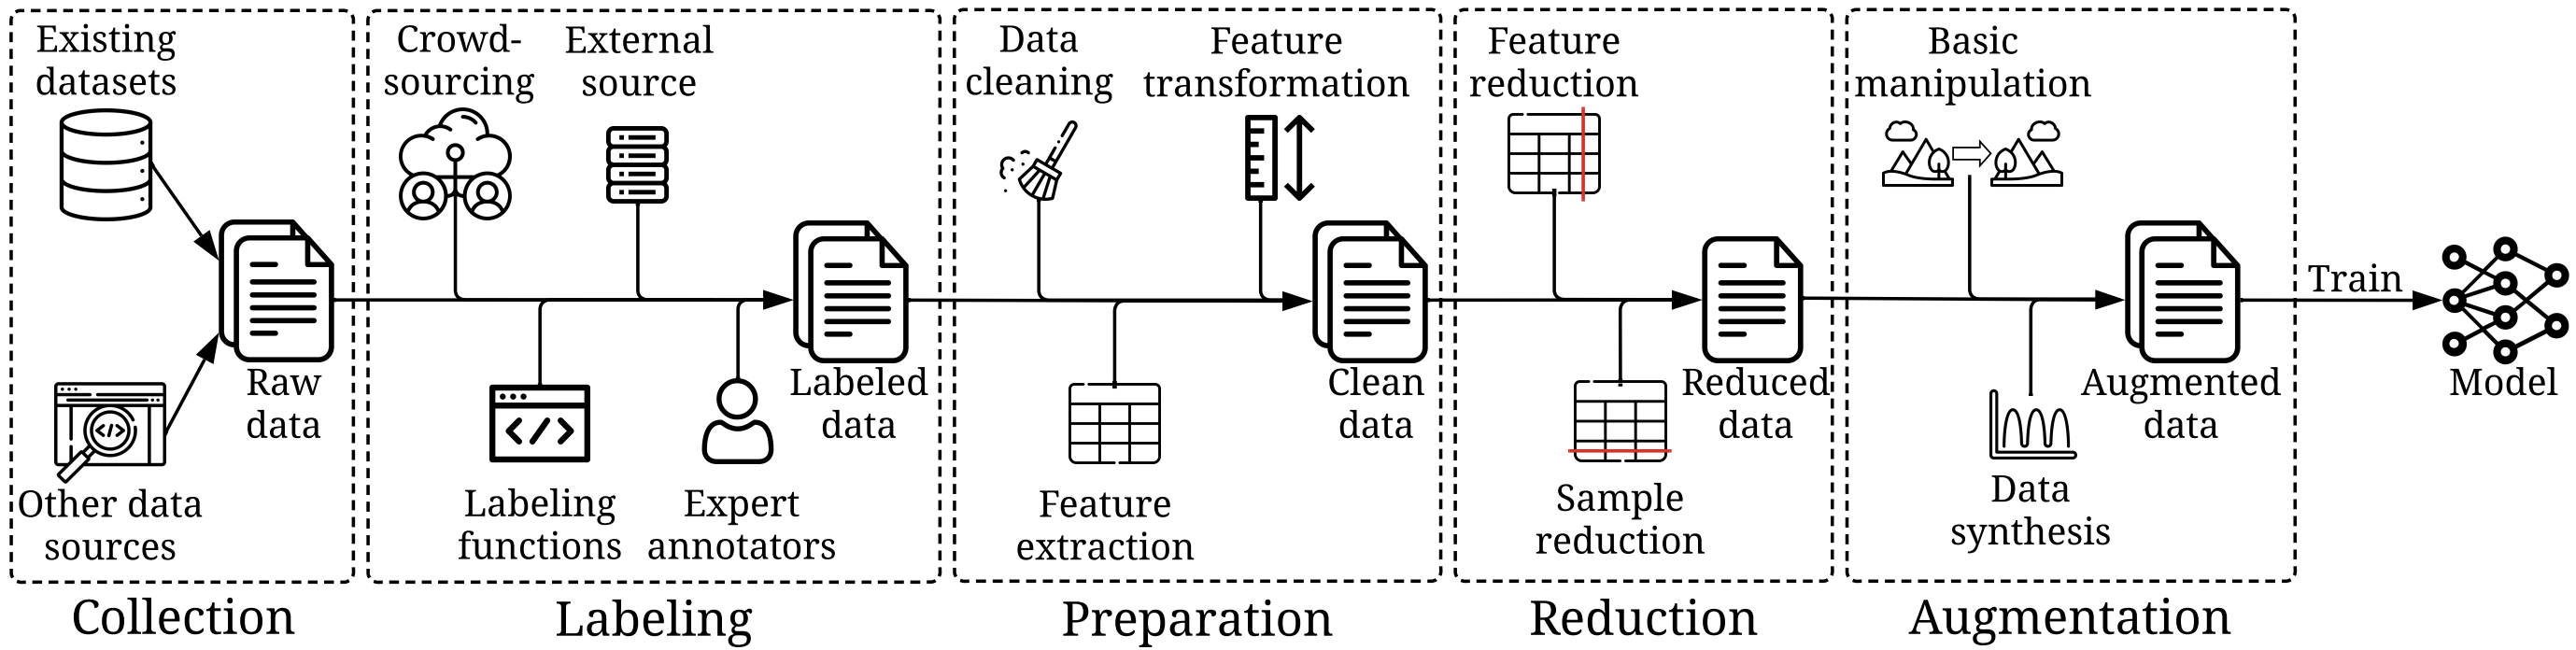
\includegraphics[width=1\textwidth]{images/datacentric.png}
    \caption{https://arxiv.org/pdf/2303.10158}
   \label{fig:lenet}
\end{figure}

As seen from the previous figure training data development in data-centric AI is divited to five sub-goals: collection, labeling, preparation, reduction and augmentation. However this sub-goals can be executed in different order or some of them can be skipped. [https://arxiv.org/pdf/2303.10158]. For example in this work real data is collected, prepared, reducted and labeled in following order. For synthetic data it is collected by generating, reducted and then labeled. Implementations of these subgoals are presented in following sections.


%In first sub-goal it is needed to mapping what is needed to trainin. In online there is various datasets available for different use cases, even pre-trained models. Sometimes existing datasets are not suitable for the task and it is needed to create own dataset. 


%In second sub-goal raw training data is labeled. Labeling is the process where the data is annotated with the correct labels. Crowdsourced labeling is very usual in labeling process as it can divide labeling task to smaller parts. In crowdsoured labeling traditionally labeling guidelines are given to annotators. It is important that guidelines are clear that annotations will be consistents even it is labeled by different annotators. For consistent annotations it can be used pre annotation task where same samples are annotated based on guidelines and evaluating results. One other way could be doing small pilot where iteratively improving guidelines. Semi-supervised learning is a method where the model is trained using both labeled and unlabeled data.

%In third sub-goal raw training data is prepared

%In fourth sub-goal raw training data is reduced.

%In fifth sub-goal raw training data is augmented.

\begin{table}[ht]
    \begin{tabular}{|l|r|r|r|r|}
    \hline
    Model & Precision\textsubscript{IoU:50} & Recall\textsubscript{IoU:50} & F1\textsubscript{IoU:50} & AP\textsubscript{IoU:50-95} \\
    \hline
    s500 & 0.482 & 0.924 & 0.634 & -\\
    s1000 & 0.740 & 0.901 & 0.813 & - \\
    s1500 & 0.787 & 0.892 & 0.836 & - \\
    s2000 & 0.854 & 0.883 & 0.869 & - \\
    s2500 & 0.847 & 0.848 & 0.848 & - \\
    \hline
    \hline
    yolov8n (Base) & 0.877 & 0.657 & 0.751 & - \\
    \hline
    \end{tabular}
    \caption{Comparisons of fully trained YOLOv8n models and the base model} 
    \label{tab:results}
    \end{table}


    \begin{table}[!h]
    \centering
    \begin{tabular}{|c|c|c|}
    \hline
    Model & Realease date & image generation method \\ \hline
    AlignDRAW & 2015 & \\ \hline
    DALL-E & 2021 & Autoregressive \\ \hline
    DALL-E 2 & 2022 & Diffusion \\ \hline
    Midjorney & 2022 &  \\ \hline
    Stable diffusion& 2022 & \\ \hline
    Stable diffusion XL & 2023 & \\ \hline
    FLUX.1 & 2024 & Diffusion \\ \hline

    %https://arxiv.org/html/2403.11614v4
    %Underwater Mine-like Object Detection & images generated via the Diffusion Mode & \\ 

    %https://arxiv.org/abs/2410.12953

    %" GANs to generate realistic synthetic data not only increases the diversity and quantity of training data but also improves the adaptability of the object detection model to the complexities and variations in real industrial scenarios" 
    \end{tabular}
    \caption{Summary of text-to-image models.}
    \label{tab:models}
    \end{table}

    \begin{figure}
    \centering
    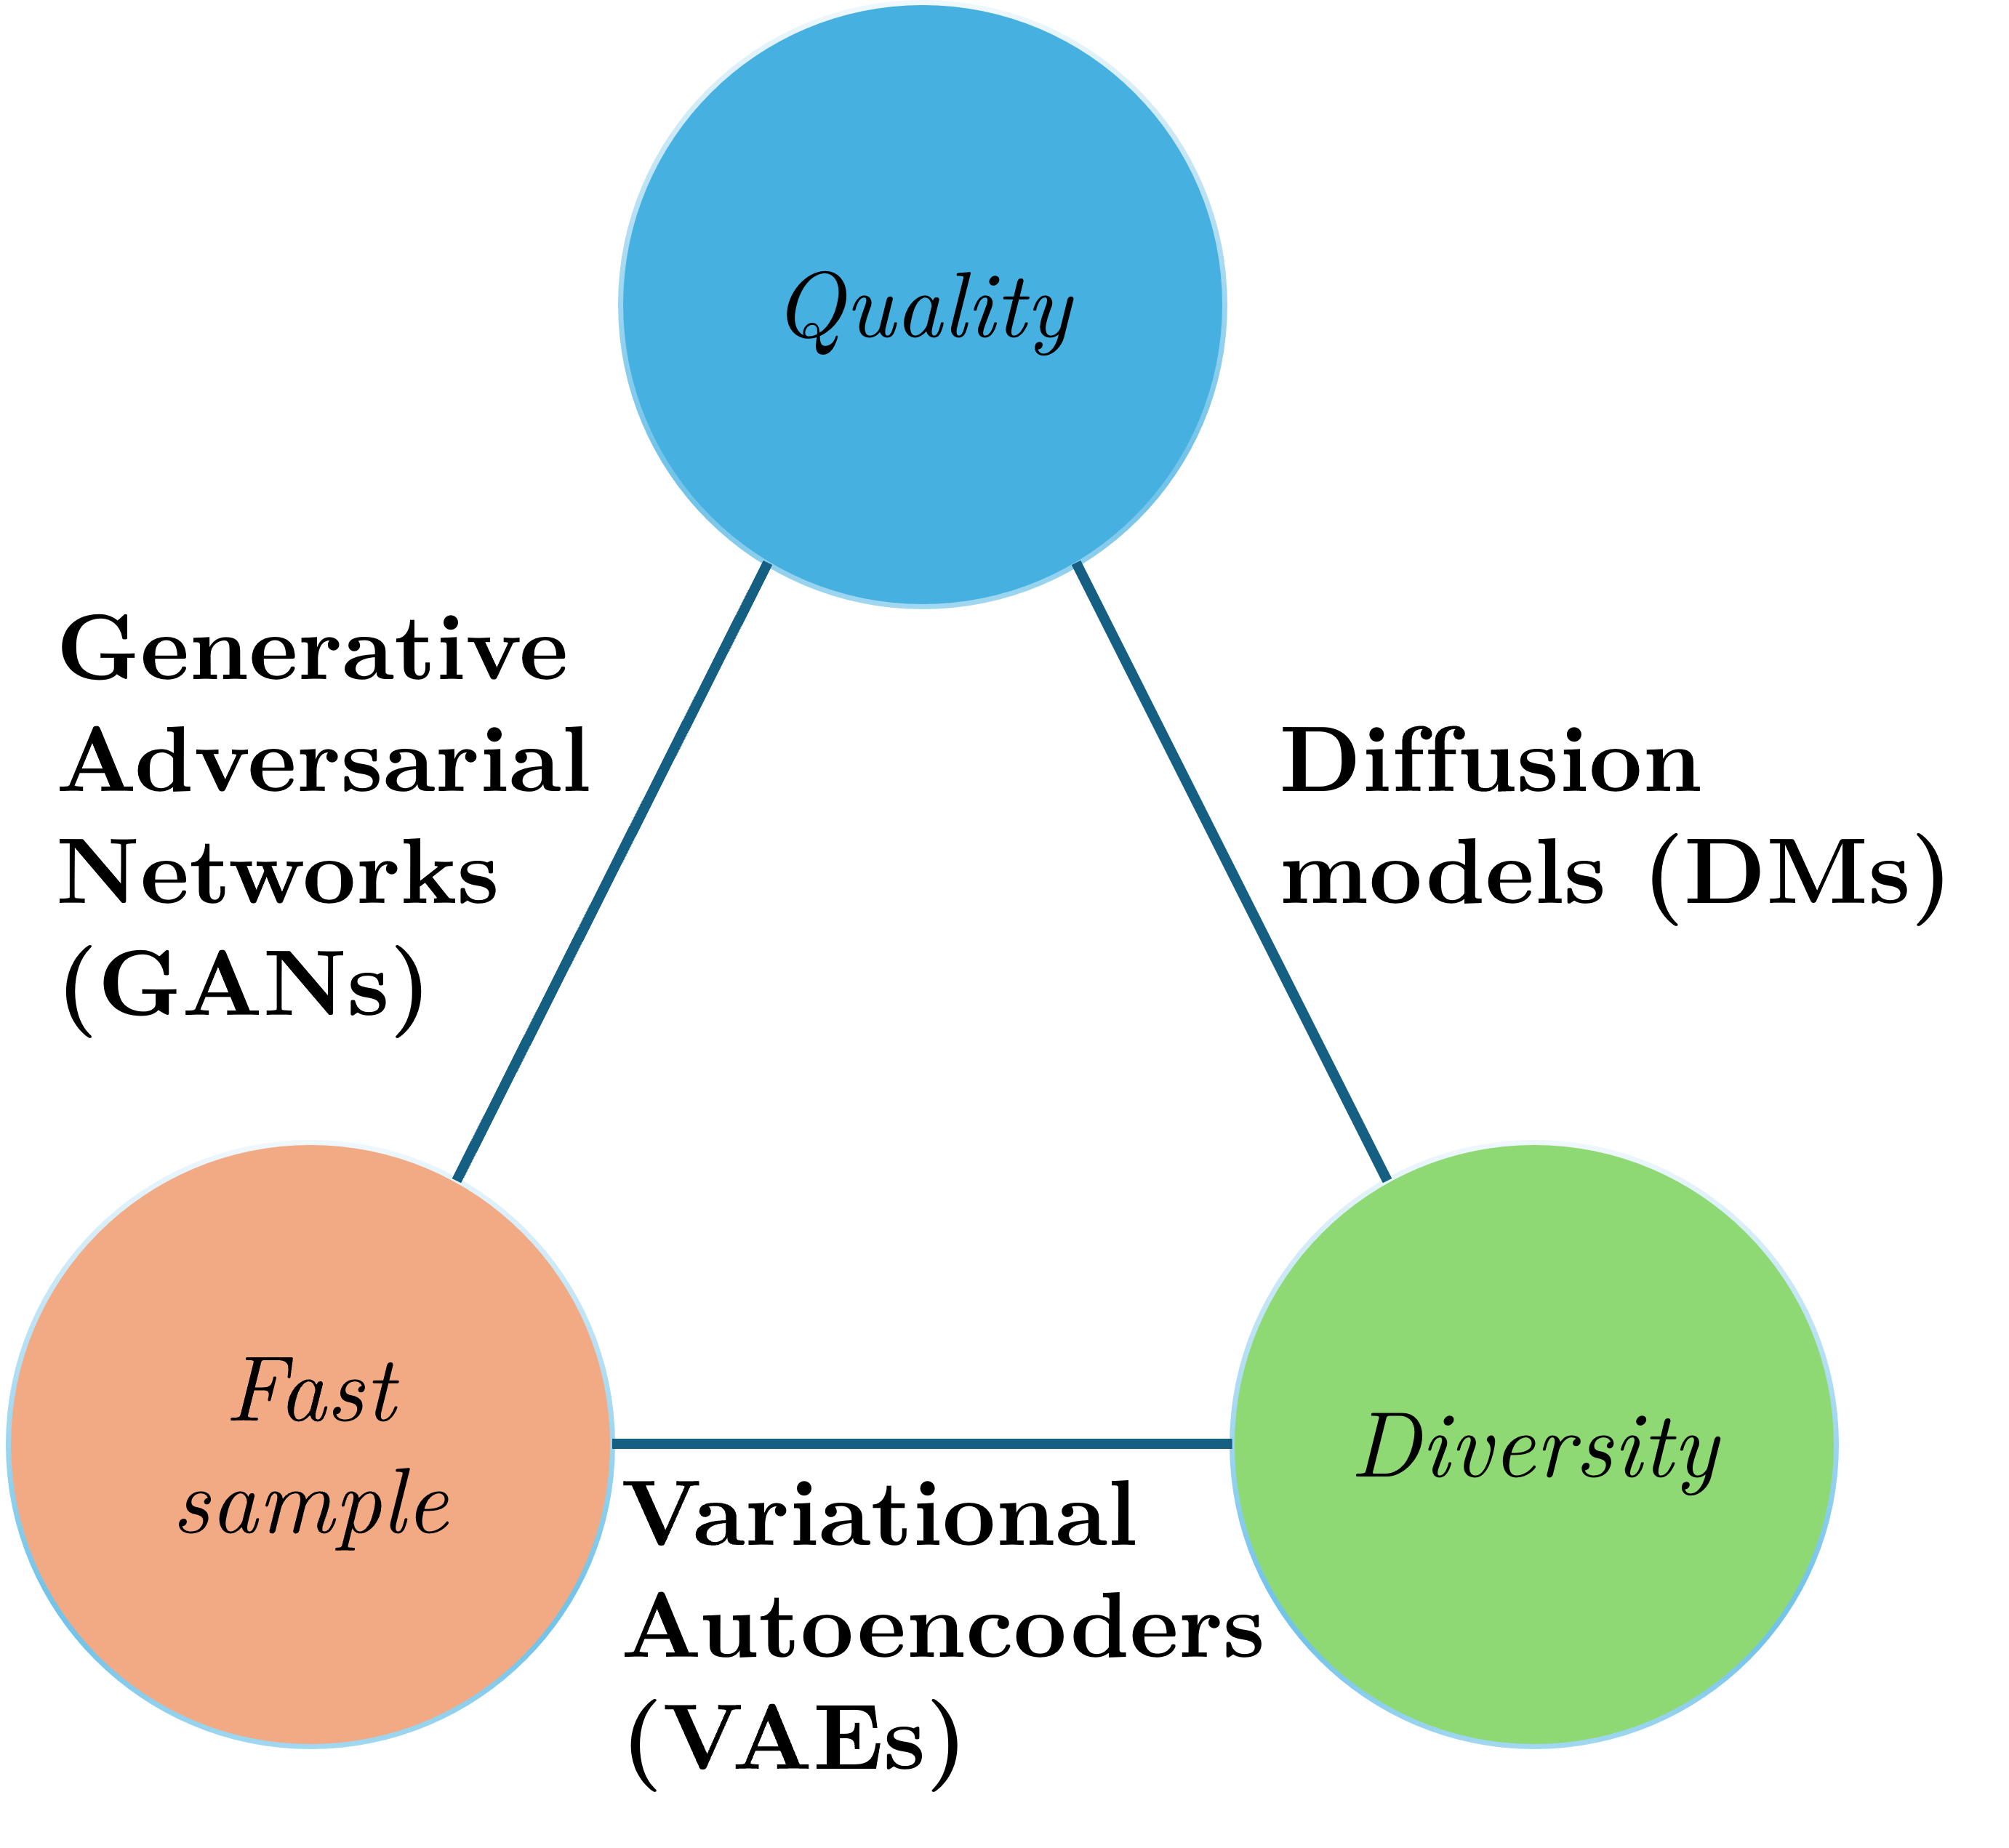
\includegraphics[width=0.7\textwidth]{images/background/txt2img/Kuva5.png}
    \caption{-}
   \label{fig:diffusion_process}
\end{figure}
%Image cations - bla bla -- made by author
Ge


Text-to-image (T2I) models can generate images based given textual description [Text-to-image Diffusion Models in Generative AI: A Survey] combining so fields of computer vision and natural language processing [Text-to-Image Synthesis: A Decade Survey]. As the case is generation the main aim is generate new high-quality images instead than retrieving existing ones. Many modern T2I models are capable of generating high-quality images with good text-image consistency and more complex textual prompts by large-scale training on millions of image-text pairs. 

Modern T2I generation starts from 2015 when Elman Mansimov's team introduce AlignDRAW. It was capable show relationship between text input and generated images by using attention mechanism even though it’s results was not so realistic. [Text-to-Image Synthesis: A Decade Survey] [Text-to-image Diffusion Models in Generative AI: A Survey]. After 2015 T2I made great progress by introduction of Generative Advesarial Networks (GANs) which followed many variation of GAN models like StackGAN, AttnGAN and CP-GAN. In 2021 OpenAI introcuced DALL-E, autoregressive (AR) model which utilized tranformer architecture and large-scale dataset to generating  diverse scale of high-quality images even it suffering high computational cost. Now in resent years diffusion methods (DM) like DALL-E 2 or FLUX.1 has become very popular and becoming leading method in T2I generation. Latent diffusion models (LDM) like Stable Diffusion, which will be in the center of this thesis, not only improved quality of generated images but also reduced computational cost by operating in latent space instead of pixel space.



Next section will be not introduced other T2I models other than diffusion-based methods as they are not in the main focus of this thesis. To read more about T2I models like GANs or AR models, see papers[] and [].

\begin{table}[h!]
    \centering
    \scriptsize
    \begin{tabular}{p{2cm}|p{3cm}|p{3cm}|p{2cm}|p{2cm}|p{1.5cm}}
    \hline
    \textbf{Technique} & \textbf{Study Focus} & \textbf{Synthetic Image Generation Method} & \textbf{Performed well with synthetic data only} & \textbf{Performed better with synthetic and real data than only using real data} & \textbf{Reference} \\ \hline \hline
    3D simulation & Arbitrary objects for Robot perception & iPhone 3D scans and NVIDIA Omniverse Isaac Sim & Yes & Maybe (not only real data case included in training) & \cite{singh2024syntheticalargescalesynthetic}\\ \hline

    3D simulation & Traffic vehicles detection & Domain randomization using 3D models & Yes & Yes & \cite{tremblay2018trainingdeepnetworkssynthetic} \\ \hline

    3D simulation and Text2img & Aerial ship detection & Unity and Stable Diffusion with different domain adaption algorithms & Maybe & Not used real data in training & \cite{app14114558} \\ \hline

    Image blending & Arbitrary objects in indoor scenes & Object placement and blending into real photos & No & Yes & \cite{georgakis2017synthesizingtrainingdataobject} \\ \hline

    Image blending & Milk package detection in refrigerator & Object placement and blending into real photos & No & Yes & \cite{Bartolovic2024FromST} \\ \hline

    Img2img & Aerial transmission tower and tower components detection & Synthetising images using the AirSim simulator and Unreal Engine and adapt those to be more realistic using CycleGAN, CUT, and TSIT & Yes & Yes & \cite{Peterlevitz2023SimtoRealTF} \\ \hline

    Img2img & Industrial object detection & CycleGAN-based model with two generators and two discriminators & Yes & Yes & \cite{math11224588} \\ \hline

    Text2img & Aerial object detection & Fine-tuning Stable Diffusion model & Not tested & Yes & \cite{jian2023stablediffusionaerialobject} \\ \hline

    Text2img & Downstream road detection & Fine-tuning Stable Diffusion model & Yes & Yes & \cite{tang2024crsdiffcontrollableremotesensing} \\ \hline

    Text2img & Heavy machinery detection and classification & DreamBooth framework with Stable Diffusion XL (SDXL) & No & Yes & \cite{xin2024dartautomatedendtoendobject} \\ \hline

    Text2img & Motorcyclists' helmet violation detection & Convolutional generative adversarial networks (DCGANs) & Not tested & Yes & \cite{a17050202} \\ \hline

    Text2img & Skin disease classification & Stable diffusion & Yes & Yes & \cite{akrout2023diffusionbaseddataaugmentationskin} \\ \hline

    Text2img & Traffic vehicles detection and classification in urban application & Kandinsky 2.2 diffusion model & Maybe & Not used real data in training & \cite{REUTOV2023335} \\ \hline

    Text2img & Underwater Mine-like Object Detection & Comparison of synthetic data generation methods, including GANs and diffusion models (DDPM and DDIM) & Yes & Yes & \cite{agrawal2024syn2realdomaingeneralizationunderwater} \\ \hline
    \end{tabular}
    \caption{Summary of studies focusing on syn2real problem in object detection.}
    \label{tab:syn2realtable}
\end{table}

   %From papers listen in table common trend was also boost of the performance when using even small amount of real data with synthetic data. Some papers found fine-tuning on real data after training on synthetic data improved performance, but cases where there was not enough real data, simultaneos training was more effective.

    %In paper \cite{burdorf2022reducingrealworlddata} used two aproaces to training object detection model: pretrained model with synthetic data and then fine-tuned on real data and model trained with mixed datased of synthetic and real data. In the paper there was not found significant difference between these two approaches. Also they estimated that in mixed dataset most reduction of real data is using 5\%-20\% ratio of real data in synthetic data.

    The motivation to use synthetic data is mainly related with difficulties to collect large and diverse dataset for training object detection model \cite{voetman2023bigdatamythusing}. Common reasons for supplementing a dataset with synthetic data include an insufficient amount of real data, lack of public datasets, or the absence of pretrained models for similar use cases. As capturing of real data can have several difficulties like high cost of capturing data, time-consuming labeling and privacy conserns can synthetic data alleviate the challenges of training object detection models. \cite{kiefer2021leveragingsyntheticdataobject, Delussu2024synthetic, nguyen2024application} For example synthetic data generating can, depending on the used method, produce fastly and cheaply great amount of data and auto-labeling them \cite{kiefer2021leveragingsyntheticdataobject, nguyen2024application}. Also with synthetic data it is possible to simulate rare scenarios and objects that are not appered in real datasets making so possible to train model detect edge cases \cite{Zhang2024, edgecases}. However when only simulated or synthetic data is used to train object detection model for real-world applications, models performance is usually lower than using real-world data for training. This happens because input distripution has shifted between synthetic and real data. [https://arxiv.org/html/2403.04114v1] 
Synthetic-to-real (syn2real) or simulation-to-real (sim2real) gap are terms that are often used in literature when researching how to close the gap between synthetic and real data.

%Starting from the informative region selection, the Integral Image of the input image is calculated, where each pixel value is the sum of the pixel values in the rectangle formed by the top-left corner and the pixel's location. This method provided faster calculation in constant time to compute Haar-like features, which are rectangular patterns of contrasting regions.

%After that, multiple different scaled sliding windows are used to detect features as features work with different scaling or locations. For detection, combined classifiers in a cascade are used to classify whether the window contains objects. These cascade of classifiers are trained each increasingly difficult example of positive (face) and negative (non-face) image samples with the learning algorithm AdaBoost. Classifiers in the cascade go through the simplest to the more complex classifiers and stop immediately if the current classifier gives a negative outcome based on given extracted Haar-like features. This makes it very efficient as false negative cases are discarded quickly, leaving more computation time for more promising regions where objects might be.

% If comparing AP and F1-score, AP has information about precision and recall trade-off in all confidence score thresholds, while F1-score is only one point in the precision-recall curve. In the other words AP depends only fixed IoU threshold while  F1-score also depends used confidence threshold score. Based on this it is desited in this work that AP is used main evaluate metric to measure overall  performance for trained object detection models, while F1-score is used to find the optimal confidence score threshold for the models.  


%Next as demonstrate how the step shows, the VJ detector is chosen for closer observation as it was considered a turning point in the history of object detection.

%The VJ detector is an object detection algorithm used to detect human faces without constraints. What makes it very remarkable in the history of object detection is that it worked in real-time at 15 frames per second on a 700MHz Pentium III CPU \cite{object_detection_review}\cite{object_detection_20years}.


%The main idea is to extract Haar-like features from the image and use several classifiers to find out is region face or not. Haar-like features are rectangular patterns of constracting regions. To extract these fast, a single grayscaled input image is first converted to Integral image. Integral image is repersentation where each pixel value is the sum of the origal images pixel values in the rectangle formed by the top-left corner of the image and the pixel's location. This method provides computing Haar-like features in constant time at any location or scale. 
%There is several classifiers in VJ detector that are trained with AdaBoost learning algorithm. Each classifier is trained with positive (face) and negative (non-face) image samples with increasing difficulty. These classifiers are then combined in a cascade where each classifier looks more features compared to previous ones. This makes it very efficient as likely non-face cases are discarded quickly, leaving more computation time for more promising regions where objects might be.
%In detection pipeline image is scanned by detector with various scales and locations and at each scan Haar-like features are computed using integral image. Each sub-image from detector is evaluated by cascade of classifiers. Classifier accesses and computes the necessary Haar-like features for sub-image using the integral image. Based on extracted features from sub-image if the current classifier gives a negative outcome, the process stops immediately. If sub-image passes all classifiers, it is classified as a face.[https://www.cs.cmu.edu/~efros/courses/LBMV07/Papers/viola-cvpr-01.pdf] 
%This text gives a general picture how VJ detector works discarding some details like variance normalization for minimize the effect of illumination changes.  


% Definition for good object detection models depends it's designed use case. For example, a model used in a surveillance camera might need high speed and low computational cost, while in medical imaging high accuracy and precision are more important. There is many different ways to observe how good object detection model is: Model accuracy to detect correctly objects, performing well different conditions and how scalable model for retraining. Also computational performance, low error rate with predictions and working with edge cases are also... To create a good object detection model it needed to take several factors into account like choosing most fitting object detection method, quality and size of the training dataset and possible preprocessing teqniques.

%EDIT SEMI-AI TEXT TO OWN


What makes a good object detection model generally depends on its intended use case. For example, a model deployed in a surveillance camera may require high speed and low computational cost, whereas in medical imaging, high accuracy are more critical. When generally comparing object detection algorithms usually they are evaluated with classification metrics like average precision (AP) but also other metrics like inference speed, and model size using typical benchmark datasets like COCO (Common Object In Context) \cite{lin2015microsoftcococommonobjects, algocomp, yolo11-docs,xin2024dartautomatedendtoendobject}. When training model for own use there can be there can be several criteria by which the quality of an object detection model can be evaluated like robustness under varying conditions, scalability for retraining or the ability to handle certain edge cases. Training a good object detection model requires multiple factors, such as selecting a suitable object detection model to train with, ensuring the quality and size of the training dataset, and applying appropriate preprocessing techniques.

What makes a good object detection model generally depends on its intended use case. For example, a model deployed in a surveillance camera may require high speed and low computational cost, whereas in medical imaging, high accuracy is more critical. When comparing object detection algorithms, they are usually evaluated with classification metrics like average precision (AP), but also with other metrics such as inference speed and model size, using benchmark datasets like COCO (Common Objects in Context) \cite{lin2015microsoftcococommonobjects, algocomp, yolo11-docs, xin2024dartautomatedendtoendobject}. There can also be several case-dependent criteria for evaluation when training a model that are needed to take into account while planning and testing model like scalability for retraining or the ability to handle certain edge cases. To training a good object detection model requires handling with several factors, that usually includes selecting a suitable object detection model, providing a training dataset with appropriate size and quality, and applying preprocessing techniques.


%As explained with plain language how attention is computed by vectors: the query asks which keys have important information for it, the keys answer which of them are important to the query, while also possessing the information that is stored in the value. After the query gets answers from the keys, it weights the each keys information from the values according to the importance determined by the keys.


As explained first these three vectors role to calculate attention them and attention first simplified way, Query is the one that seeks important information from other embeddings which are in this case keys. First query asks which keys has important information (which is value in this case). Then keys answers which one of them are important to query also giving the information that keys posses. After the query getting answers from keys, query weighting information based on importance that key had


Self-attention mechanism is the most important part of the transformer architecture as it captures relationships and dependencies between embeddings. For each embedding vector in the sequence there is created three different vectors: query $Q$, key  $K$ and value  $V$. 
Query represents the one certain element in the sequence and key one embeddings in the sequence against the query. Key-query pairs are used to calculate attention score, which determines how relevant key element is to the query in the current context. As key-query holds information about relevansy between query and key element, value vector has information where to move in embedding space that encodes the meaning of the 

%The role of query, key and value matrices it to extract relevant information from the embedding vectors for their tasks. (Hideya Mino et al., 2017)
%Meaning of matrices: The role of query and key matrices is to select relevant entity for search operation and value matrix is pull out relevant features for retrieval.
% Value matrix encodes the context representations 
%features from the embedding vectors that is needed for their tasks.
%[https://arxiv.org/pdf/2110.09419]
%The role of matrices in attention mechanism is to extract relevant features from selected entities,

%https://www.ethansmith2000.com/post/softmax-attention-is-a-fluke

%[https://arxiv.org/pdf/2310.07323].

%value of words are not fixed, as same words can have several different values in vector space. but they can their value can be changed by attention mechanism. For example value for word "Rock" get meaning from other words in the sequence as it can meand music genre or stone based on context. This is a part where attention mechanism used to move the initial embedding of the particular word to the direction giving its contextual meaning.

%Even words can has multiple meaning like word "Rock" can mean stone or music genre, complex meanings can be linked to the context as embedding space is large enough. NOT TRUE. VECTOR HAS BASE VALUE AND ATTENTION MECHANISM CHANGES VALUE TO GIVE CONTEXTUAL MEANING.



%In text-to-image generation or natural language processing words are usually encoded as word vectors (aka. word embeddings). These numerical vectors are reprecentation of words that are also captures semantic meaning. For example words like  "car" , "vehicle" and "truck" are close in the vector space. Also relationships between words can be encoded between distances like if word vector of word "king" distracting "man" and then adding vector "woman" it should be give vector for word "queen". Word vectors are denoted as $v_i \in \mathbb{R}^{1 \times D} $ where $i$ is index of the certain word and $D$ is dimension of vector. Words are first tokenized as giving each word unique index $i$. 

%Embedding vectors captures semantic meaning and relationship of tokens in embedding space making possible guiding other modalities.  In textual data this means that words with similar meaning, like "car" and "vehicle", are close to each other in the embedding space. Also relationships between words can be seen as vector distance. For example distance between "France" and "Paris" is similar to distance between "Finland" and "Helsinki" encoding so "capital of" relationship. However polysemous words like ""rock" that can mean sotne or music genre, can get its contextual meaning by attention mechanism where initial embedding value is adjusted based other embedding in the sequence.

%maybe about pros and cons of each method



%As seen paper above synthetic data generated with certain methdos can help to solve problem with insufficient amount of data. Also synthetic data can helpfull with other things besides increasing dataset. Controlability to create new scenarios and rare situations that might not be in real datasets is usually possibly in simulations which helps increase variety of using dataset. Also some methods providing possibility for automated labeling top of rapid generation of the synthetic images.



    
  
    %Also [paper] showed potential of diffusion models generate noisy  leading to more diverse and generalizable datasets. That 

    %At the start of working thesis sevaral approaches was considered. For example simulating unity would be good because you can randomize people position and poses. Still if used generate images surface normal, NIR or color, there was a lot of off ass synthetic data does not had artifact like real sensor had. It comes to mind to preprocess real data or simulate artifacts top of synthetic images. After that comes mind can image generators teached to learn produce style of images with its artifacts.

    %In this work our interest is in text-to-image generation as it has generate rare image formats like sonar images in [paper]. 
    %nvidia inpaint 3dmodels to photolike using stable diffusion, 



% 2x2 grid of images as example: 3d simulation, diffusion model-based synthetic image generation, object blending into images

% example image missdetect cat as a dog. Grad-cam shows that model made decision based cat's face and people face what was next to it. instead to solve promple making dataset more diverse by adding more cat and dog images, it should be including more images where cat and dog are together with people.

\begin{figure}
    \centering
    
\includegraphics[width=0.5\textwidth]{images/q.png}
    \caption{Images of extracted features from different layers of CNN. Low-level features shows edges and corners and high-level features shows more abstract features. }
%    https://www.researchgate.net/figure/
%A-common-widely-shared-example-illustrating-how-neural-networks-learn-hierarchical_fig1_335360163}
   \label{fig:CNN_featurs}
\end{figure}

%4When training the neural network that generates the parameters in equation \ref{eq:reverse_process}, it takes input sample $x_t$ and time step $t$ in order to account for the variance schedule of the forward process. Since different time steps correspond to different noise levels, the model must learn to denoise each step individually. 
%As the objective is to learn the distribution of the training data it is needed to maximise the likelihood that model is given for $x_0$. To do so it is needed to marginalise over from T to down 1 and calculate loss function, in this case largest log likelihood i.e $\log (p_{\boldsymbol{\theta}}(x_0))$,
%but as it would require integrating over all possible trajectories from noise to the data manifold it is intractable.Even though it can't optimize that loss function directly, it can optimize a variational lower bound which indirectly also optimizes the intractable loss function.

%In this work used dataset are collected from our recordings. Recordings are done by using near infrared sensor (NIR) which gives 1-channeled grayscale images. For further use, grayscale images are converted to 3-channeled RGB images by allocating same grayscale value to each channel.

%As interest for generating synthetical images for different image format comparet general RGB, infrared images are used.

%IR-images are saved as PNG files for faster processing and smaller memory size compared...
%Also images are saved in 3 channeled RGB format where each channel has same grayscale\dots

%As covariance matrix $\beta_{t} \mathbf{I}$ is diagonal, noise will be independetly and identically distributed as standard normal for each pixel and so gaussian noise will be isotropic.
%more about non isometric noise https://arxiv.org/pdf/2210.12254

%https://freedium.cfd/https://medium.com/@steinsfu/diffusion-model-clearly-explained-cd331bd41166

%and likelyhood of $x_0$ is related to all reverse steps through the chain rule:

%\begin{equation}
%    p_{\boldsymbol{\theta}}\left(x_0\right)=\int p_{\boldsymbol{\theta}}\left(x_{0:T}\right) \, dx_{1:T} \,.
%    \label{eq:likelihood}
%\end{equation}

%By maximising likelihood of equation \ref{eq:likelihood} it is possible to learn conditional probabilities $p_{\boldsymbol{\theta}}\left(x_{t-1} \mid x_t\right)$. \cite{strümke2023lecturenotesprobabilisticdiffusion} 

%In \cite{ho2020denoisingdiffusionprobabilisticmodels} it desided experimentally reverse process variance $\boldsymbol{\Sigma}_{\boldsymbol{\theta}}\left(\mathbf{x}_t, t\right) = \sigma_t^2 \mathbf{I}$ to be $\sigma_t^2 = \tilde{\beta}_t = \frac{1-\bar{\alpha}_{t-1}}{1-\bar{\alpha}_{t}}\beta_t$ instead of $\sigma_t^2=\beta_t$. Now $L_{t-1}$ can be written as

%For training to predict the noise it is usually used U-Net architecture.
%Cross-attention and self-attention maps in each layer of U-Net. Cross-attention maps carries semantic information of the text prompts, while self-attention maps preserve spatial information as it helps each pixel to see relevance of other pixels in the image \cite{liu2024understandingcrossselfattentionstable, app1409371}. 

%Algorithms \ref{alg:training_ddpm} and \ref{alg:sampling_ddpm} are based on the original DDPM paper \cite{ho2020denoisingdiffusionprobabilisticmodels}. There is also other approaches to implement diffusion models like DDIM (Denoising Diffusion Implicit Models) which is a non-Markovian variant of DDPM that allows for fewer sampling steps and faster inference \cite{song2020denoisingdiffusionimplicitmodels}.


%Buckets are used to group different sized images and then process them to fit buckets resolution size during training. However, as all images were same size and there was no need to use buckets for different sized images, it was decided to upscale images before training.



%Upscaling can also do later with same tool that is used to training LoRA. Buckets are containers for different image sizes as in training different sized images can't be trained as the same time. If there is only same sized images Bucket are not nesessary. However it is possible set bucket resolution and upscale images in the bucket. It was desided to upscale manually as every image were same size and it gives freedom to choose end size of the image.


%\item \textbf{Buckets (Kohya SS)}:  Integrated resizing method in Kohya SS LoRA training tool (more information in table \ref{tab:explanationloraparams}). The idea is test how scaling by using buckets differs from direct pixel scaling in image generation.

%MUOKKAA ---- In this work ControlNet is not used, but it is playing important role works where real or similations images are tried to be transformed 


%In typical text-to-image models with classifier-free guidance CLIP text encoder encodes text into image-text embedding space. Then these embeddings are injected into U-Net architecture of diffusion model via cross-attention mechanism where image features acts as query and text embeddings as key and value.
%Cross-attention and self-attention maps in each layer of U-Net. Cross-attention maps carries semantic information of the text prompts, while self-attention maps preserve spatial information as it helps each pixel to see relevance of other pixels in the image \cite{liu2024understandingcrossselfattentionstable, app1409371}. In sampling process 

%In practise input prompt is encoded into text embeddings using CLIP text encoder. These text embeddings are injected into U-net via cross-attention mechanism where image features acts as query and text embeddings as key and value.

%CLIP consists of two pre-trained encoders: image encoder (f.ex Vision Tranformer or ResNet) and text encoder (f.ex Text Transformer or CBOW).

%For example image synthesis process can be conditioned by text, images, even visual signals like depth maps or sketches. These conditioning methods can be used for instance text-to-image generation, inpainting or generating image from visual signals. \cite{zhan2025conditionalimagesynthesisdiffusion} In the text-to-image generation main approach to implement condition mechanism is to use guidance methods. and one that has become mainsteam condition approach in Diffusion-based Conditional Image Synthesis (DCIS), classifier-free guidance. 

%This work will be centered discussing theory around textual conditioning via CLIP model which is used in stable diffusion model.

%The most basic attempt to implement textual conditioning goes following way: text prompt $y$ are encoded tokens and feed into a transformer model to get embeddings. In U-net there is attention layer for each layer in the U-Net. Embedding are then concatenated to the attention context at attention layers to attend to use information of text prompt during image generation. However, this approach itself not generate images that clearly match with text needing other aproach to give stronger signal from the text-prompting. \cite{strümke2023lecturenotesprobabilisticdiffusion} To solve this problem there is used classifier guidance or and more popular one classifier-free guidance.  

%In this case it means model learns from text-image-pairs. \cite{strümke2023lecturenotesprobabilisticdiffusion}

%CLIP tranformerihin -  CLIP model used in latent diffusion model is trained using 400 million image-text pairs from internet public datasets.

%Jotain kertomaan hieman etukäteen mihin tätä käytetään työssä?


%removed part about how u-net and text encoder affects. %chen2024enhancingdiffusionmodelstextencoder
%https://huggingface.co/blog/sdxl_lora_advanced_script

%In addition to giving image-caption pairts for training there is about 150 different hyperparameters that can be edited. Most important hyperparameters were summarized in the table \ref{tab:explanationloraparams}, while used training hyperparameters are in the table \ref{tab:basicloraparams}.

%To further investigate the impact of captions it was traied two LoRAs with same hyperparameters, one with  and one without captions. Based on generating images using same parameters and different seeds, it showed that no captioning model mimiced well monocromic characteristics of the orginal image but it was not flexible and contollable from promps. For example including different objects or using negative prompts prevent object from training data was less effective when captions was not used in training.

%KUVA neljä kuvaa, jossa toisessa negative prompt toimii paremmin kuin toisessa

%For example in training dataset there appeared multiple times a person with a beanie. In no-caption LoRA it was difficult to prevent generating people with beanie, but in captioned LoRA (where beanie was mentioned in captions) it was easier to control using negative prompts.



%Afterwards there was published some papers that also support some of the community findings:

%\begin{itemize}
%    \item Precision (how accurate the caption describes what is in the image) is more important in captioning than recall (how well the caption covers all relevant aspects of the image). More diverse details in captions enchance performance and prevent halluciantion. \cite{cheng2024precisionrecallanalysisimage}
%    \item Accurate annotation is important. Captions should first aim for precision and reliability before adding details, and then include only as much detail without being too lengthy or overly detailed. \cite{wang2025harnessingcaptiondetailnessdataefficient}
%\end{itemize}
    
%Even though these papers were not focused directly focused for LoRA training, findings support the idea that captions should be accurately describe the most important features, without being too long and detailed.

%These hyperparameters produced LoRA models that generated images visually similar to the original NIR images when adapted to SDXL. 
% As scope of this work was create a pipeline from scratch only improving dataset, there was not done extensive hyperparameter tuning.

%As results the LoRA model used for training captured well orginal characteristics of the training dataset which can be seein in the figure \ref{lora_weight_comparison}.

%This configuration was sufficient to capture the monochromatic characteristics of the NIR sensor images without overfitting.

%Some papers also shows YOLOv8n having best tradeoff between model size and accuracy\cite{xin2024dartautomatedendtoendobject}. 


%The thesis has three main objectives:
%1. Reviewing existing methods to generate synthetic images and their effectiveness to improve performance of object detection models. Based on the review, diffision-based text-to-image model is chosen for implementation.
%2. Implementing from scratch a complete synthetic data and object detection pipeline using open-source tools and models.
%3. Analysing the effect of different combinations of real and synthetic data on the performance of the object detection model and mirroring results from the literature. 



%In this work there was researched three main objectives:
%1. Literature review about can the object detection model be improved by using synthetic images and what methods there is to generate synthetic images (Chapter 2).
%2. Implementation of the synthetic data generation and object detection pipeline from scratch based on the literature review. (Chapter 3)
%3. Compare object detection models trained with different combinations of real and synthetic data each other and results from literature. (Chapter 4)


It should be also taken into account that some cases in \textit{“Performed better with synthetic and real data than only using real data”} were not compared with the same sized real dataset which might distort the results.

while other sections cover the theoretical background for object detection, deep learning and diffusion based text-to-image models.

In this thesis, it was hypothesized that even though the synthetic data is not completely similar to real data, it still looks very similar to real data and so can be used to give more realistic information about an object's features. Based on this, the first research question is formulated as follows: Can the object detection model be improved by using synthetic images generated from a fine-tuned text-to-image model in training? To answer this question, the text-to-image model will first be fine-tuned by training a Low-rank adaptation (LoRA) model using 31 different real images. After that, by using the fine-tuned text-to-image model, similar images will be generated as if they were taken from a sensor camera. As an additional interest, it will be tested how well the text-to-image model can be controlled by text prompts to generate different scenarios, like including different objects that did not exist in the original dataset. In the end, the object detection model will be trained with synthetic and real images to see how well it can detect objects from real images.

The research subject for this thesis is people detection in images taken from a Near Infrared (NIR) sensor. This topic is chosen because it is straightforward to experiment with from scratch. Also, image representation from the NIR sensor is assumed to be uncommon in pretrained object detection models, and it had provided NIR sensor recordings of people small space at the start of the thesis work.

%Chapter 2 is divided three main topics. First, the theoretical background about object detection and deep learning. Second sim-to-real problem and third text-to-image models.

%KUVAAN ja kuvaukseen OTA MALLIA   Training Deep Networks with Synthetic Data: Bridging the Reality Gap by Domain Randomization
%Jonathan Tremblay, Aayush Prakash, David Acuna, Mark Brophy, Varun Jampani, Cem Anil, Thang To, Eric Cameracci, Shaad Boochoon, Stan Birchfield Nvidia

%SImilar results about seed relation irregularities was got when r400s1000 and r400s1500 was retrained once with new shared seed.  As results, when in Figure~\ref{fig:detection_results} r400s1000 (AP 0.938) outperformed r400s1500 (AP 0.921), in retrained models r400s1500 (AP 0.932) outperformed r400s1000(AP 0.30). 

aulukosta voidaan nähdä että eniten FP and FN tapauksia YOLOv8n base modelin predictioneissa. Kun base modelia fine-tuunattiin synteettisillä sekä oikeilla kuvilla. false tapaukset vähenivät huomattavasti.   Alla olevasta kuvasta \ref{fig:yolov8n_detections} on esitettynä esimerkkejä YOLOv8n mallin tekemistä tunnistuksista rajoitetusta määrästä testikuvia (including 4 recordings), koska suostumusta saada näyttää ei ollut myönnetty kaikkiin kuviin.

\begin{figure}[ht]
\centering
% Row 1
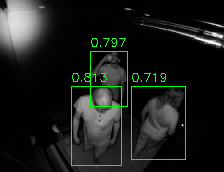
\includegraphics[width=0.32\textwidth]{images/results/yolov8n/onnistuneet/royale_20240710_110402_frame198.png}
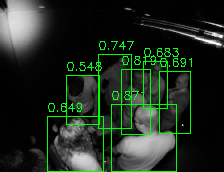
\includegraphics[width=0.32\textwidth]{images/results/yolov8n/onnistuneet/royale_20240710_110908_frame147.png}
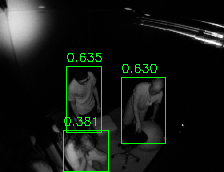
\includegraphics[width=0.32\textwidth]{images/results/yolov8n/onnistuneet/royale_20240710_110908_frame261.png}\\[4pt]
% Row 2
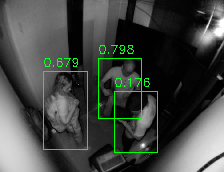
\includegraphics[width=0.32\textwidth]{images/results/yolov8n/onnistuneet/royale_20240710_130444_frame327.png}
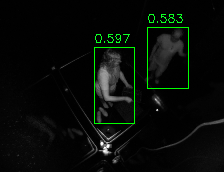
\includegraphics[width=0.32\textwidth]{images/results/yolov8n/onnistuneet/royale_20240710_134224_frame1098.png}
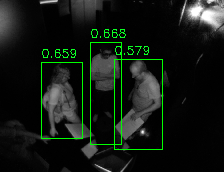
\includegraphics[width=0.32\textwidth]{images/results/yolov8n/onnistuneet/royale_20240710_141816_frame519.png}
\caption{Six  YOLOv8n base model with IoU 0.5 and optimised confidence threshold.}
\label{fig:yolov8n_tp}
\end{figure}

Tarkasteltaessa tarkemmin yolov8n mallin tekemiä predictioneita testikuvista suoraan, voitiin nähdä mallin pärjäävän pääsäntöisesti hyvin perustapauksissa, jossa ihminen oli selkeästi näkyvissä sisältäen sekä erikoistapaukset joissa ihminen oli erityisen lähellä kameraa. Kumminkin joissain tiloissa ja katselukulmasta malli sattoi olla havaitsematta ihmisiä hyvin usein vastaavanlaisia aikaisempia perustapauksissa, mikä koostaa suurimman osan FN tapauksista. Lisäksi erityisesti tapaukset joissa ihminen oli lattialla, lähellä toisiian tai tilan suuaukon lähettyvillä, malli ei tunnistanut ihmisiä. Vastaavasti FP virhehavaintoja tuli usein jos henkilöllä oli kantamuksia tunnistaen kantamuksien peittoavan osan perusteella ihmisen monessa osassa tai havaitsemalla ihmiseksi myös ihmisiä ympäröivän tilan.

\begin{figure}[ht]
\centering
% Row 1
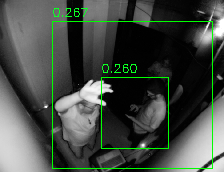
\includegraphics[width=0.32\textwidth]{images/results/yolov8n/virhe/royale_20240710_130444_frame549.png}
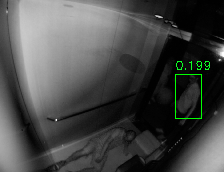
\includegraphics[width=0.32\textwidth]{images/results/yolov8n/virhe/royale_20240710_113404_frame387.png}
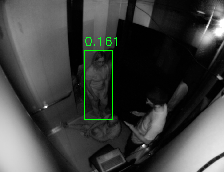
\includegraphics[width=0.32\textwidth]{images/results/yolov8n/virhe/royale_20240710_130444_frame201.png}\\[4pt]
% Row 2
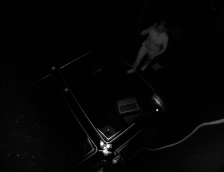
\includegraphics[width=0.32\textwidth]{images/results/yolov8n/virhe/royale_20240710_134224_frame1071.png}
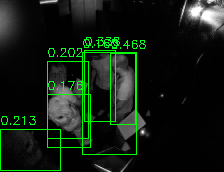
\includegraphics[width=0.32\textwidth]{images/results/yolov8n/virhe/royale_20240710_141816_frame690.png}
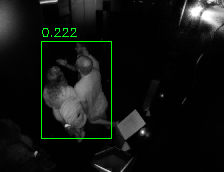
\includegraphics[width=0.32\textwidth]{images/results/yolov8n/virhe/royale_20240710_141816_frame747.png}
\caption{YOLOv8n: epäonnistuneet/virheelliset havainnot (FN/FP), 6 satunnaista esimerkkiä.}
\label{fig:yolov8n_fnfp}
\end{figure}

Verraten tapauksia s2000 ja r568s2500 malleihin, mallit tunnistavat pääasiassa kaikki perustapaukset. Vaikka ongelmia oli edelleen tunnistaa lattialla tai poikkeavissa asennoissa olevia ihmisiä, näiden tunnistamisessa oli selvä parannus verraten YOLOv8n base modeliin. Lisäksi ympäristöä ei tunnistettu virheellisesti ihmiseksi. Kumminkin poiketen base modelista merkittävä osa FP tapauksista malli tunnisti usein kädet erikseen ihmiseksi, jos ne olivat korostetusti esillä kun sensoria koskettaessa tai pitäessä käsiä suorassa ylhäällä (mahdollisesti labelöinnin syy).


\begin{figure}[ht]
\centering
% Row 1
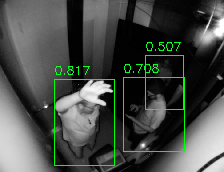
\includegraphics[width=0.32\textwidth]{images/results/r568s2500/compare/royale_20240710_130444_frame549.png}
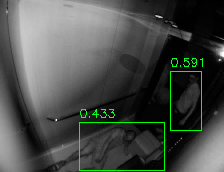
\includegraphics[width=0.32\textwidth]{images/results/r568s2500/compare/royale_20240710_113404_frame387.png}
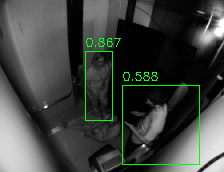
\includegraphics[width=0.32\textwidth]{images/results/r568s2500/compare/royale_20240710_130444_frame201.png}\\[4pt]
% Row 2
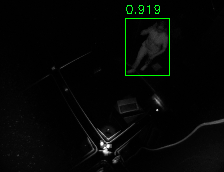
\includegraphics[width=0.32\textwidth]{images/results/r568s2500/compare/royale_20240710_134224_frame1071.png}
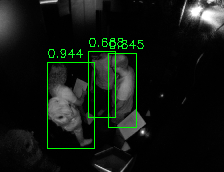
\includegraphics[width=0.32\textwidth]{images/results/r568s2500/compare/royale_20240710_141816_frame690.png}
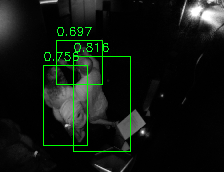
\includegraphics[width=0.32\textwidth]{images/results/r568s2500/compare/royale_20240710_141816_frame747.png}
\caption{r568s2500 vastaavat havainnot kuin YOLOv8n kuvassa \ref{fig:yolov8n_fnfp} }
\label{fig:fine_fnfp}
\end{figure}

\begin{figure}[ht]
\centering
% Row 1
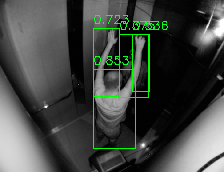
\includegraphics[width=0.49\textwidth]{images/results/r568s2500/kasi/royale_20240710_130444_frame909.png}
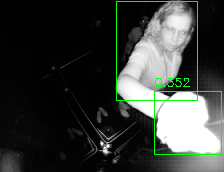
\includegraphics[width=0.49\textwidth]{images/results/r568s2500/kasi/royale_20240710_134224_frame1146.png}
\caption{Virheellisesti tunnistetut kädet ihmiseksi r568s2500 mallissa.}
\label{fig:fine_kasi}
\end{figure}

For all the models the optimal confidence thresholds to achieve the best F1-scores were calculated and the results are shown in the table below.


Tärkeinpinä havointaina voitiin nähdä, että puhtaasti synteettisillä kuvilla hieno säädetty malli pärjäsi huomattavasti paremmin kuin base model ja sisällymällä suhteellisen pienen määrän aitoja kuvia synteettisten kuvien joukkoon, pystyttiin saavuttamaan vielä parempi suorituskyky, kunhan synteettisiä kuvia oli riittävän paljon.

Loppuhavointona voitiin, todeta synteettisen data ei ainoastaan parantanut mallin suorituskykyä, mutta

Tärkeinpinä havaintoina voitiin nähdä, että synteettisen datan määrä korreloi pääsääntöisesti mallin suorituskyvyn kanssa.

Saadut tulokset osoittivat selvästi, että

\begin{table}[ht]
\centering
\renewcommand{\arraystretch}{1.15}
\setlength{\tabcolsep}{8pt}
\begin{tabular}{|l|r|r|r|r|r|}
\hline
Model & Ground-truth & Predictions & TP & FP & FN \\ \hline
s2000      & 1785 & 1702 & 1542 & 160 & 243 \\ \hline
r568s2500  & 1785 & 1714 & 1591 & 123 & 194 \\ \hline
YOLOv8n    & 1785 & 1496 & 1207 & 289 & 578 \\ \hline
\end{tabular}
\caption{Ground truth, predictions, true positives (TP), false positives (FP), and false negatives (FN) for selected models (IoU = 0.50) using optimized confidence thresholds.}
\label{tab:selected_models_counts}
\end{table}


This work is structured as follows. Chapter 2. Chapter 3 details the scope of this work, implemented end-to-end pipeline for synthetic data generation and object detection, and fine-tuned object detection models. Chapter 4 compares the fine-tuned object detection models. Chapter 5 discusses and analyses the results and suggests future work. Chapter 6 concludes the work.

\textbf{Synthetic image generation}

Työn tuloksista voidaan nähdä, että toteutetuilla tavoilla pystyttiin tuottamaan visuaalisesti uskottavia synteettisiä kuvia. Kuitenkin parannettavaa löytyy vielä. Esimerkiksi välillä kuvien generoinnissa joutui käyttäämään isompiakin vahvuuksia prompeissa, jotta jotkut toistuvat elementit opetuskuvista ei esiintyisi kovin usein. Vaikka kuvia ei olisi paljoa LoRAn kouluttamiseen, jatkossa vieläkin määrää tärkeämpää olisi kuvien olevan erilaisia keskenään kuten ympäristö, ihmiset ja sekä mahdollisesti muut muuttuvat tekijät vaihtuisi mahdollisimman paljon. Oletuksena on että malli pystyisi tuottamaan vieläkin erilaisempia kuvia helpommin, ilman että tietyt asiat puskisi selvästi muita enemmän. Vaikka tässä työssä tarkasteltiin esimerkiksi yläperspektiivistä hissitiloissa, uskottavasti mallin suorituskyky myös hyötyisi, jos opetuskuvat sisältäsi näistä poiketen jonkin verran esimerkiksi lähikuvia, straight-on kuvia tai kuvia aivan eri ympäristöistä kuten käytävistä tai auloista. Tietenkin tällöin captioning merkitys korostuu, jotta nämä voidaan erottaa toisistaan.

\textbf{Future works}


Tulevaisuuden töissä yksi keskeisimpiä kehityksen kohteita olisi selvittää voidaanko synteettisen kuvat annotoida jo niiden luontivaiheessa, sillä tämä poistaisi manuaalisen annotoinnin tarpeen saaden kuvat mahdollisesti heti käyttöön. Esimerkiksi Diffusion Attentive Attribution Maps (DAAM) \cite{https://arxiv.org/pdf/2210.04885} menetelmällä voidaan tuottaa heatmap kuvia, jotka näyttävät mihin kohtiin generoitua kuvaa malli kiinnitti huomiota tietyn prompotin, esimerkiksi "ihminen", suhteen. Tätä menetelmää yhdessä esimerkiksi segmentanything \cite{https://arxiv.org/pdf/2304.02643, https://huggingface.co/spaces/Xenova/segment-anything-web} mallin kanssa mahdollistaisi todennäköisesti hyvinkin tarkan automaattisen bounding boxien luomisen suurimmalle osalle generoiduille kuville. Työn lopussa tehtyjen kokeilujen perusteella segmentanything toimi hyvin synteettisien kuvien kanssa.

Muita tutkimuskohteita voisi olla työn eri vaiheiden optimointi, kuten caption menetelmien vertailu (esim. hyvin pitkät täsmälliset vs. lyhyet ytimekkäät), tai upscaling approaches and quantitatively evaluating the fidelity between generated and real images using metrics such as Fréchet Inception Distance (FID), Kernel Inception Distance (KID), or Inception Score (IS)

%\begin{table}[ht]
%    \centering
%    \begin{tabular}{|p{0.17\textwidth}|p{0.10\textwidth}|}
    \hline
    Model \newline(s = synthetic,\newline\hspace*{0.1em} r = real)  & 
    ~ \newline {AP\textsubscript{IoU:50}} \\
    \hline
    s500 & 0.866 \\
    s1000 & 0.888 \\
    s1500 & 0.889 \\
    s2000 & 0.908 \\
    s2500 & 0.876 \\
    \hline
    r200 & 0.828 \\
    r200s500 & 0.862 \\
    r200s1000 & 0.893 \\
    r200s1500 & 0.915 \\
    r200s2000 & 0.920 \\
    r200s2500 & 0.922 \\
    \hline
    r400 & 0.854 \\
    r400s500 & 0.909 \\
    r400s1000 & \textbf{0.938} \\
    r400s1500 & 0.921 \\
    r400s2000 & 0.925 \\
    r400s2500 & 0.932 \\
    \hline
    r568 & 0.923 \\
    r568s500 & 0.929 \\
    r568s1000 & 0.916 \\
    r568s1500 & 0.917 \\
    r568s2000 & 0.921 \\
    r568s2500 & \textbf{0.938} \\
    \hline
    \hline
    yolov8n (Base) & 0.815 \\
    \hline
%   \end{tabular}
%    \caption{Comparisons of fine-tuned YOLOv8n models with freezed-layers and the base model} 
%    \label{tab:results}
%    \end{table}



    \begin{sidewaystable}[ht]
    \begin{tabular}{|l|r|r|r|r|r|r|r|r|r|r|r|r|r|r|r|r|r|}
    \hline
    Model & GT BB & Prediction BB & TP\textsubscript{50} & FP\textsubscript{50} & FN\textsubscript{50} & Precision\textsubscript{50} & Recall\textsubscript{50} & F1\textsubscript{50} & Best Threshold\textsubscript{50} & TP\textsubscript{75} & FP\textsubscript{75} & FN\textsubscript{75} & Precision\textsubscript{75} & Recall\textsubscript{75} & F1\textsubscript{75} & Best Threshold\textsubscript{75} & AP\textsubscript{50-95} \\
    \hline
    s500 & 1785 & 3419 & 1649 & 1770 & 136 & 0.482 & 0.924 & 0.634 & 0.770 & 1329 & 2090 & 456 & 0.389 & 0.745 & 0.511 & 0.839 & 0.625 \\
    s1000 & 1785 & 2175 & 1609 & 566 & 176 & 0.740 & 0.901 & 0.813 & 0.640 & 1359 & 816 & 426 & 0.625 & 0.761 & 0.686 & 0.798 & 0.633 \\
    s1500 & 1785 & 2023 & 1592 & 431 & 193 & 0.787 & 0.892 & 0.836 & 0.633 & 1338 & 685 & 447 & 0.661 & 0.750 & 0.703 & 0.756 & 0.632 \\
    s2000 & 1785 & 1846 & 1577 & 269 & 208 & 0.854 & 0.883 & 0.869 & 0.384 & 1322 & 524 & 463 & 0.716 & 0.741 & 0.728 & 0.728 & 0.634 \\
    s2500 & 1785 & 1787 & 1514 & 273 & 271 & 0.847 & 0.848 & 0.848 & 0.621 & 1310 & 477 & 475 & 0.733 & 0.734 & 0.733 & 0.653 & 0.636 \\
    \hline
    r200 & 1785 & 4433 & 1615 & 2818 & 170 & 0.364 & 0.905 & 0.519 & 0.849 & 1199 & 3234 & 586 & 0.270 & 0.672 & 0.386 & 0.875 & 0.258 \\
    r200s500 & 1785 & 2016 & 1508 & 508 & 277 & 0.748 & 0.845 & 0.793 & 0.505 & 1266 & 750 & 519 & 0.628 & 0.709 & 0.666 & 0.706 & 0.588 \\
    r200s1000 & 1785 & 1989 & 1572 & 417 & 213 & 0.790 & 0.881 & 0.833 & 0.460 & 1335 & 654 & 450 & 0.671 & 0.748 & 0.707 & 0.568 & 0.441 \\
    r200s1500 & 1785 & 1858 & 1574 & 284 & 211 & 0.847 & 0.882 & 0.864 & 0.392 & 1360 & 498 & 425 & 0.732 & 0.762 & 0.747 & 0.620 & 0.521 \\
    r200s2000 & 1785 & 1940 & 1629 & 311 & 156 & 0.840 & 0.913 & 0.875 & 0.639 & 1369 & 571 & 416 & 0.706 & 0.767 & 0.735 & 0.740 & 0.557 \\
    r200s2500 & 1785 & 1787 & 1584 & 203 & 201 & 0.886 & 0.887 & 0.887 & 0.323 & 1361 & 426 & 424 & 0.762 & 0.762 & 0.762 & 0.604 & 0.589 \\
    \hline
    r400 & 1785 & 3088 & 1635 & 1453 & 150 & 0.529 & 0.916 & 0.671 & 0.763 & 1370 & 1718 & 415 & 0.444 & 0.768 & 0.562 & 0.798 & 0.563 \\
    r400s500 & 1785 & 2010 & 1569 & 441 & 216 & 0.781 & 0.879 & 0.827 & 0.547 & 1356 & 654 & 429 & 0.675 & 0.760 & 0.715 & 0.675 & 0.609 \\
    r400s1000 & 1785 & 2021 & 1660 & 361 & 125 & 0.821 & 0.930 & 0.872 & 0.657 & 1422 & 599 & 363 & 0.704 & 0.797 & 0.747 & 0.774 & 0.574 \\
    r400s1500 & 1785 & 1867 & 1618 & 249 & 167 & 0.867 & 0.906 & 0.886 & 0.441 & 1379 & 488 & 406 & 0.739 & 0.773 & 0.755 & 0.627 & 0.586 \\
    r400s2000 & 1785 & 1820 & 1601 & 219 & 184 & 0.880 & 0.897 & 0.888 & 0.261 & 1392 & 428 & 393 & 0.765 & 0.780 & 0.772 & 0.612 & 0.599 \\
    r400s2500 & 1785 & 1921 & 1645 & 276 & 140 & 0.856 & 0.922 & 0.888 & 0.549 & 1422 & 499 & 363 & 0.740 & 0.797 & 0.767 & 0.689 & 0.607 \\
    \hline
    r568 & 1785 & 2035 & 1633 & 402 & 152 & 0.802 & 0.915 & 0.855 & 0.571 & 1363 & 672 & 422 & 0.670 & 0.764 & 0.714 & 0.727 & 0.609 \\
    r568s500 & 1785 & 1789 & 1579 & 210 & 206 & 0.883 & 0.885 & 0.884 & 0.258 & 1367 & 422 & 418 & 0.764 & 0.766 & 0.765 & 0.578 & 0.636 \\
    r568s1000 & 1785 & 1863 & 1593 & 270 & 192 & 0.855 & 0.892 & 0.873 & 0.520 & 1390 & 473 & 395 & 0.746 & 0.779 & 0.762 & 0.604 & 0.615 \\
    r568s1500 & 1785 & 1827 & 1587 & 240 & 198 & 0.869 & 0.889 & 0.879 & 0.355 & 1353 & 474 & 432 & 0.741 & 0.758 & 0.749 & 0.566 & 0.620 \\
    r568s2000 & 1785 & 1789 & 1597 & 192 & 188 & 0.893 & 0.895 & 0.894 & 0.280 & 1383 & 406 & 402 & 0.773 & 0.775 & 0.774 & 0.664 & 0.626 \\
    r568s2500 & 1785 & 1809 & 1622 & 187 & 163 & 0.897 & 0.909 & 0.903 & 0.426 & 1407 & 402 & 378 & 0.778 & 0.788 & 0.783 & 0.603 & 0.632 \\
    \hline
    \hline
    yolov8n & 1785 & 1337 & 1172 & 165 & 613 & 0.877 & 0.657 & 0.751 & 0.252 & 1028 & 309 & 757 & 0.769 & 0.576 & 0.659 & 0.294 & 0.603 \\
    \hline
    \end{tabular}
    \caption{Object Detection Results}
    \label{tab:results}
    \end{sidewaystable}

    \begin{table}[ht]
\centering
\begin{tabular}{|p{2cm}|p{1cm}|p{1cm}|p{1cm}|p{1cm}|p{1cm}|p{1cm}|p{1cm}|p{1cm}|p{1cm}|}
\hline
Model & Best Threshold & Total gt & Total pred & TP & FP & FN & Precision & Recall & F1 \\ \hline
s500         & 0.770 & 1785 & 1747 & 1455 & 292 & 330 & 0.833 & 0.815 & 0.824 \\ \hline
s1000        & 0.593 & 1785 & 1748 & 1527 & 221 & 258 & 0.874 & 0.855 & 0.864 \\ \hline
s1500        & 0.498 & 1785 & 1789 & 1540 & 249 & 245 & 0.861 & 0.863 & 0.862 \\ \hline
s2000        & 0.384 & 1785 & 1702 & 1542 & 160 & 243 & 0.906 & 0.864 & 0.884 \\ \hline
s2500        & 0.369 & 1785 & 1654 & 1485 & 169 & 300 & 0.898 & 0.832 & 0.864 \\ \hline
r200         & 0.818 & 1785 & 1780 & 1384 & 396 & 401 & 0.778 & 0.775 & 0.776 \\ \hline
r200s500     & 0.505 & 1785 & 1531 & 1395 & 136 & 390 & 0.911 & 0.782 & 0.841 \\ \hline
r200s1000    & 0.398 & 1785 & 1670 & 1496 & 174 & 289 & 0.896 & 0.838 & 0.866 \\ \hline
r200s1500    & 0.392 & 1785 & 1622 & 1499 & 123 & 286 & 0.924 & 0.840 & 0.880 \\ \hline
r200s2000    & 0.441 & 1785 & 1750 & 1585 & 165 & 200 & 0.906 & 0.888 & 0.897 \\ \hline
r200s2500    & 0.180 & 1785 & 1771 & 1590 & 181 & 195 & 0.898 & 0.891 & 0.894 \\ \hline
r400         & 0.659 & 1785 & 1973 & 1520 & 453 & 265 & 0.770 & 0.852 & 0.809 \\ \hline
r400s500     & 0.577 & 1785 & 1604 & 1458 & 146 & 327 & 0.909 & 0.817 & 0.860 \\ \hline
r400s1000    & 0.609 & 1785 & 1705 & 1574 & 131 & 211 & 0.923 & 0.882 & 0.902 \\ \hline
r400s1500    & 0.311 & 1785 & 1738 & 1577 & 161 & 208 & 0.907 & 0.883 & 0.895 \\ \hline
r400s2000    & 0.228 & 1785 & 1749 & 1582 & 167 & 203 & 0.905 & 0.886 & 0.895 \\ \hline
r400s2500    & 0.469 & 1785 & 1721 & 1580 & 141 & 205 & 0.918 & 0.885 & 0.901 \\ \hline
r568         & 0.566 & 1785 & 1646 & 1540 & 106 & 245 & 0.936 & 0.863 & 0.898 \\ \hline
r568s500     & 0.195 & 1785 & 1746 & 1587 & 159 & 198 & 0.909 & 0.889 & 0.899 \\ \hline
r568s1000    & 0.350 & 1785 & 1723 & 1564 & 159 & 221 & 0.908 & 0.876 & 0.892 \\ \hline
r568s1500    & 0.338 & 1785 & 1694 & 1555 & 139 & 230 & 0.918 & 0.871 & 0.894 \\ \hline
r568s2000    & 0.218 & 1785 & 1734 & 1591 & 143 & 194 & 0.918 & 0.891 & 0.904 \\ \hline
r568s2500    & 0.332 & 1785 & 1714 & 1591 & 123 & 194 & 0.928 & 0.891 & 0.909 \\ \hline
yolov8n      & 0.161 & 1785 & 1496 & 1207 & 289 & 578 & 0.807 & 0.676 & 0.736 \\ \hline
\end{tabular}
\caption{Comparisons of trained YOLOv8n models with optimised confidence threshold}
\label{tab:object_detection_metrics}
\end{table}


the results are presented for different fine-tuned YOLOv8n object detection models that were trained by using different ratio of synthetic and real images. These models are compared to YOLOv8n basemodel with evaluation metrics of interest. The later part of the section presents discussion about optimal synthetic/real ratio based on the results from the first part of the section. Also optimised threshold is calculated for best performing model from first part of the section and it's evaluation metrics is presented.

Based on the chapter section \ref{sec:object_detection_evaluation_metrics}, it is used AP as main metric to evaluate models overall performance. 
After evaluating the models, it will be selected the best performing models and...


Saadut tulokset osoittivat selvästi, että työn menetelmillä tuotetuilla synteettisillä kuvilla voidaan parantaa hahmontunnistusmallin suorituskykyä. 

Esimerkiksi huolimatta siitä että keskiarvo r568 malilla oli matalampi kuin päätuloksissa, ei olisi ihmeellistä että lisätyt kuvat r400 mallin päälle paransivat huomattavasti mallin suorituskykyä. Syynä voi olla esimerkiksi se, että lisättyt kuvat 

Tuloksissa havaita poikkeuksellista vaihtelua joidenkin mallien suorituskyvyn suhteen päätuloksissa perusteltiin kouluttamalla muutama malli uudelleen, mutta eri seediä käyttäen. Varsinaista ylioppimista ei havaittu mallien koulutuksen aikana, sillä training ja validation tappiofunktioiden käyrät olivat molemmat laskevia

Nämä vaihtelut juontavat syväoppimisen mallien koulutuksen stokastisesta luonteesta. Kuten sectionissa \ref{sec:CNN} on kuvattu, neurovekko oppii painot erottamaan hyödylliset piirteet kuvista sekä luokitelemaan ne korkea-dimensioisella fully connected leyaers, joita sitten päivitetään iteratiivisesti koulutuksen aikana.  Tämä luo erittäin monimutkaisen systeemin, jossa pienet muutokset opetus datasetissä, painojen alustuksessa tai hyperparametreissä voivat johtaa toissa tapauksessa ylioppimiseen tunnistaen heikosti uusia tapauksia ja toisessa laadukkaaseen malliin oppien erottelemaan juuri tarpeellisen informaation kohteen tunnistamiseen liittyen.

Tarkasteltaessa vain käytetän datan näkökylmasta todennäköisyys että kuinka paljon saman mallin eri lopputulokset eroavat toisistaan käymään riippuu vahvasti sen puoleen käytetyn datasetin laadusta ja sen koosta. Esimerkiksi 
yksipuolisessa datasetissä mallin on vaikea mallia tapauksille saa haastetta joutua luomaan joustava malli tunnistaa kohde näistä erilaisissa olosuhteissa. Vataavasti tarpeeksi iso datasetissä ei ole vain todennäköisemmin eri tapauksia joista  malli oppii piirteitä, mutta yksittäisen kuvan vaikutus pienenee muiden kuvien kesken, jolloin malli oppii piirteet stabiilimmin.
Esimerkiksi r568 mallin keskiarvo oli korkeampi kuin s2500 mallin, mutta vastaavasti hajonta olisi paljon suurempaa. Tätä voisi selittää, että data dimensio on sama kuin kohde dimensio, jolloin malli oppii oletettavasti paremmin kohteen piirteet saaden paremman keskiarvon. Toisaalta mallin koko (ja mahdollisesti monipuolisuus) on pienempi, jolloin kuvilla on enemmän vaikutusta lopputulokseen, joka aiheuttaa suurempaa hajontaa. Kun datasetin kokoa suurennataisiin, yksittäiseen kohdistuva vaikutus pienee muiden kuvien kesken, jolloin malli oppii pirteet staabilimmin sekä kuvien uusien piirteiden kautta myös suorituskyky voi kasvaa.  


Syväoppimisessa tavoitteena on minimoida tappiofunktio, joka mittaa mallin ennusteiden ja todellisten arvojen välistä eroa. "Kaava" joka tuottaa ennusteen on koko neuroverkko painoneen, joita päivitetään iteratiivisesti koulutuksen aikana. Koska käytetyt neuroverkot ovat erittäin korkea dimensioiset ja ei-lineaariset, on olemassa monia paikallisia minimejä, joihin optimointialgoritmi voi päätyä. Tästä johtuen muutokset kuten datasetissä, hyperparametreissä tai painojen alustuksessa voivat johtaa merkittävästi erilaisiin lopputuloksiin.

Kuten taulukon päätuloksista voitiin havaita poikkeuksellista vaihtelua joidenkin mallien suorituskyvyn suhteen. Nämä vaihtelut juontavat todennäköisesti syväoppimisen mallien koulutuksen stokastisesta luonteesta. Syväoppimisessa tavoitteena on minimoida tappiofunktio, joka mittaa mallin ennusteiden ja todellisten arvojen välistä eroa. "Kaava" joka tuottaa ennusteen on koko neuroverkko painoneen, joita päivitetään iteratiivisesti koulutuksen aikana. Koska käytetyt neuroverkot ovat erittäin korkea dimensioiset ja ei-lineaariset, on olemassa monia paikallisia minimejä, joihin optimointialgoritmi voi päätyä. Tästä johtuen muutokset kuten datasetissä, hyperparametreissä tai painojen alustuksessa voivat johtaa merkittävästi erilaisiin lopputuloksiin.


Kumminkin on tärkeä muistaa, että nämä auttavat selittämään  Esimerkiksi \cite{ebadi2022peoplesanspeoplesyntheticdatagenerator} standard deviation laski kun datanmäärä kasvatettiin, mutta viimeisellä kasvatuskerralla standard deviation kasvoi moninkertaiseksi

Tästä syystä esimerkiksi sopivan monipuoliset ja erilaiset kuvat joutuvat työstämään mallia oppimaan "kaavan" jolla nämä voidaan nämäkin validointi kuvat voidaan tunnistaa, tehden paljon joustavamman mallin. Vastaavasti tarpeeksi suuri datasetti mahdollistaa saavan tarpeeksi erilaisia kuvia, jotka malli joutuu sovittamaan ja oppimaan.

The observed irregularities in the figure is likely due to the stochastic nature of training deep learning models. Tähän vaikuttaa vahvasti datasetin koko, sillä suuremmilla dataseteillä malli 

Johtuen seedin aiheuttamasta vaihtelusta. Kumminkin yleisenä neuvona voidaan sanoa, että 
Suosituksena voidaan pitää  mixed dataset with 5\%-20\% real and 80\%-95\% synthetic data \cite{burdorf2022reducingrealworlddata}. 
(power-law: https://arxiv.org/pdf/1712.00409)

Together, these findings suggest a practical guideline: even a small amount of real data, when combined with a sufficiently large set of synthetic images, can yield a more stable and better-performing model than using either data source alone.

 Tämän tuloksen on tarkoitus korostaa stocastisuuden merkitystä opetuksessa ja siten tärkeyttä testata myös mallin suorityskykyä monta kertaa eri seedeillä, jotta voidaan arvioida mallin suorituskyvyn luotettavuutta.

 Tämä kumminkin riittää osoittamaan, että synteettisillä kuvilla voidaan parantaa mallin suorituskykyä.

 Tämä esimerkiksi eroaa \cite{xin2024dartautomatedendtoendobject} saadun tutkimuksen tuloksista, jossa täysin synteettisellä dataa koulutettu yolov8n malli

 Also as usually in deep learning vision tasks performance increases logarithmically as size of the training data increases.
%https://ieeexplore.ieee.org/stamp/stamp.jsp?tp=&arnumber=8237359

From the results, it can deduces that sythetic data become more valueable when real data is scarce. It is also possible to assume that if dataset has rare scenarios that are hard to capture in real life, synthetic data can be used to cover those scenarios.

s2500 voi johtua, että malli oppii liika synteettisen datan piirteitä. 

Vaihteluille voi olla monia syitä. Esimerkiksi, vaikka koulutuksessa hyperparametrit pidettiin samoina, saaden esimerkiksi samalla datasetilla koulutettuna tuloksena samat painot, pienikin muutos datasetissä voi vaikuttaa paljonkin lopputulokseen. Esimerkiksi liikaa samankaltaisia kuvia saattaa asettua koulutuksessa niin, että malli oppii liikaa tiettyjä featureita ja ylioppminen tapahtuu heikentäen siten mallin kykyä tunnistaa kohdetta uusista kuvista. Kumminkin stokastisuus kuten se miten batch order on toteutettu, esimerkiksi satunnaisseedin kautta, voi muuttaa mallin tapaa oppia featureita eritavalla ja muuttaa tulosta huomattavasti. Tästä syystä huolellisesti koottu monipuolinen ja tarpeeksi iso datasetti mahdollistaa, että mallin ei vain oppi featureita paremmin, mutta stabiilimmin vähentäen todennäköisyyttä ylioppimiselle.
mutta ensisijaisesti todennäköisin syy tämänkaltaiselle vaihtetulle piilee koneoppimisen stokastisessa luonteessa. Vaikka käytetyt parametrit, seedid sekä kuvat olisivat samat, mutta kuvien päälle lisätään uusia kuvia, kuvien satunnainen jako batcheissä voi saada oppimaan featureita huomattavasti eri tavalla.   Esimerkiksi mallien kouluksessa stokastisuus kuten random seed ja muut vaihtelevat tekijät, vaikuttaa lopputulokseen. Esimerkiksi \cite{ebadi2022peoplesanspeoplesyntheticdatagenerator} AP:n vaihtelu mallin saman datasetin mallin, kolmen eri satunnaisseedin koulutuksessa pienemmissä suurimman ja pienimmän välinen ero oli usein 0.001-0.02 yksikköä ja suurimmillaan jopa yli 0.07 yksikköä. Vaikka
 Muita syitä, yleensä mallin suorituskyvyn laskussa, voivat olla mallin ylioppiminen, kuvien laadun heikkous, samankaltaiset ominaisuudet synteettisissä ja oikeissa kuvissa, data difficulty balance. Lisäksi suorituskyvyn poikkeuksellista kasvua vastoin AP:n kehityksen logaritmista käyrää kun kuvia lisätään voi johtua esimerkiksi, että lisätyt kuvat sisältävät jotain joka huomattavasti paranta features tunnistamista.Yleisesti kumminkin yleensä mitä suurempi ja parempi datasetti on, sitä vähemmän edellämainittua vaihtelua on odotettavissa. Tässä työssä datasetit olivat kuitenkin melko pieniä, joten figuressa esiintyvät vaihteulut voivat realistisesti mennä sattunaisuuden piikkiin.


\textbf{5.2}

From Figure~\ref{fig:threshold} it was seen that the r568s2500 model with high F1-scores across a wide range of confidence thresholds indicated more realiable detection comapared to the base model, which had vähemmän luotettavia. Tätä havaintoa tukevat esimerkiksi figureissa ~\ref{fig:yolov8n_fnfp} ja ~\ref{fig:fine_fnfp} detectionit. The relatively flat and high F1-score curve of r568s2500 model indicating having flexibility in selecting the confidence threshold, depending on whether precision or recall is prioritized. For example increasing the confidence threshold a little can be usefull if false positives are more problematic than false negatives in a given application. However best quideline is use the optimal confidence threshold that maximizes F1-score for best balance.

As seen from the detection results, even when using only synthetic data, the detection precision and recall improved significantly from the base-model. As models fine-tuned with synthetic data were able to detect people all standard cases with varying lighting conditions, it indicates that the generated synthetic images were able to overcome to domain gap to some extent. In case where hands were detected as people, it could be due the annotation of the training data as later inspection reveled that this happened also in models where only real images were used in training.
.


%discussion about results--------------------------------------------------------------

The comparison between the YOLOv8n base model and the fine-tuned r568s2500 model clearly demonstrates the positive impact of task-specific adaptation using both real and synthetic training data. The fine-tuned model exhibited substantially improved recall and precision, indicating that the synthetic data successfully complemented the limited amount of real imagery and enabled the network to learn a broader set of visual features.

The improvements suggest that synthetic data, when generated under realistic conditions and sufficient variability, can effectively enhance model robustness without requiring extensive manual data collection. The reduction in both false negatives and false positives implies that fine-tuning allowed the model to better align its learned features with the specific visual domain of the test environment.

However, several limitations were also identified. Despite the overall performance gain, the fine-tuned model occasionally produced false detections by classifying hands or partially visible limbs as separate persons. This likely originates from inconsistencies or over-segmentation in the training annotations, particularly in the synthetic dataset. Moreover, both models struggled with edge cases such as people lying on the floor or being partially occluded, highlighting the need for more diverse and pose-rich training data.

The observed variations between models also underline the stochastic nature of neural network training. Even with identical hyperparameters, small differences in training data composition or random initialization can lead to noticeable variations in the final weights and performance metrics. Consequently, when assessing model reliability, it is advisable to repeat training with multiple random seeds and report averaged metrics rather than relying on a single result.

In summary, the results support the hypothesis that fine-tuning with synthetic data can significantly improve detection performance in data-scarce scenarios. Nevertheless, achieving stable generalization requires careful dataset design, consistent annotation practices, and multiple training runs to account for stochastic effects inherent in deep learning.

\textbf{Synthetic Image Generation}

On huomioitavaa, että valittu menetelmä synteettisten kuvien tuottamiseen perustui Stable Diffusionin SDXL-mallin soveltui eritoten tutkimuskohteelle, sillä perusmalli on koulutettu pääasiassa isolla joukolla valokuvia, joissa on esimerkiksi ihmisiä, erilaisia esineitä ja ympäristöjä. Tämän vuoksi käytettyä menetelmää, jossa käytetään vain muutamaa kymmentä kuvaa mallin fine-tuunaamiseen on vaikeampi soveltaa kohteisiin jotka ovat visuaalisesti hyvin erilaisia kuin perusmallin koulutusdata. Tällaisia kohteita voivat olla esimerkiksi lääketieteelliset kuvat tai monimutkaiset teollisuuskomponentit. Toisaalta vaikkakin vastaavista kohteista on tutkimuksia, joissa käytetään tekstistä kuvaksi malleja synteettisten kuvien tuottamiseen, on näissä tapauksissa yleensä käytetty huomattavasti isompia määriä kuvia mallin fine-tuunaamiseen. Toisaalta myös muissakin tutkimuksissakin on toteutettu huomattavasti isommalla määrällä kuvia fine-tuunaus, mikä tekeekin tästä työstä poikkeuksellisen, sillä tässä työssä käytettiin vain 31 kuvaa tuottaakseen laajan joukon synteettisiä kuvia.

The results of this work show that the implemented approach was capable of producing visually convincing synthetic images. However, there is still room for improvement. For instance, during image generation, it was sometimes necessary to use stronger prompt weights to reduce the repetition of certain visual elements originating from the training images. Even when only a limited number of images are available for LoRA training, it will be even more important in future work to ensure greater diversity among them - for example, in terms of environments, people, and other varying factors. The assumption is that with more diverse training material, the model would be able to produce a wider range of images more easily, without overemphasizing recurring features.

Although in this work the generated images primarily represented elevator spaces from a top-down perspective, it is reasonable to assume that the model’s performance could further improve if the training data included a variety of other perspectives, such as close-ups, straight-on views, or entirely different environments like corridors or lobbies. In such cases, the importance of accurate and descriptive captioning becomes even more critical, as it helps distinguish these variations from one another.


\section{Discussion of implementation and results} The implementation of the synthetic data generation and object detection pipeline was successful based on the results and objectives set for this work. Työssä käytettyjen menetelmien, työkalujen ja parametrien avulla pystyttiin automatisoimaan kuvien generointi, jotka muistuttivat visuaalisesti koulutukseen käytettyjä aitoja kuvia. On huomioitavaa, että työhön valittu menetelmä tuottaa synteettisiä kuvia Stable Diffusionin SDXL-mallilla soveltui eritoten ihmisten tunnistamiseksi sisätiloista, sillä perusmalli on koulutettu pääasiassa isolla joukolla valokuvia, joissa on esimerkiksi ihmisiä, erilaisia esineitä ja ympäristöjä. Tämän vuoksi työssä käytettyä menetelmää, jossa käytetään vain muutamaa kymmentä kuvaa mallin fine-tuunaamiseen on mahdollisesti vaikeampi soveltaa kohteisiin jotka ovat visuaalisesti hyvin erilaisia kuin perusmallin koulutusdata. Tällaisia kohteita voivat olla esimerkiksi lääketieteelliset kuvat tai monimutkaiset teollisuuskomponentit. Vaikka työn toteuksen aikana on tullut paljon uusia tutkimuksia liittyen synteettisten kuvien tuottamiseen käyttäen diffuusio pohjaisia tekstistä kuvaksi malleja edellä mainittuihin esimerkkeihin liittyen, nämä jätetään tulevaisuuden tutkimuksen tarkasteluiden aiheiksi. The results demonstrated that synthetic images solely and in combination with real images can be effectively used to train object detection models for real-world images. This suggesting that generated synthetic images successfully captured the essential visual characteristics of the real domain. Relatively good and stable performance were obtained when there was a sufficient amount of synthetic images combined with real images. That effect was also seen in table~\ref{tab:ap50_seed_stats}, where s2500 model has low standard deviation, r568 higher mean and standard deviation and r568s2500 high mean and high standard derivation. It indicates that greater amount of data gives more stable results while real images can give greater boost in performance with less images comparared to synthetic images. There can be multiple reasons to explain irregulaties seen in the results along side with stochastic effects of deep learning model training. For example underperformance of s2500 model can be caused by overfitting as it was found out that while training loss decreased steadily, the validation loss started to grow on last 10 epochs. Other case for sudden high performance of r568 can be caused quality of added images as effect can be stronger as dataset's size is small. However, most of the other irregulaties can fit withing stochasticity of training where small changes such as in dataset, hyperparameters or weight initialization can lead to significantly different outcomes. This is undertandable when thinking that CNNs need to learn to extract relevant features from images and classify them with high-dimensional fully connected layers, which creates a highly complex system with many local minima in the loss landscape. From qualitative analysis it can be seen how YOLOv8n base model is familiar to detect human figures as it is very similar with monochomatic images, which can be potentially used to training the base model. However, NIR images has their own noise type and together difficult lighting conditions makes some basic cases but especially occlusions and unusual poses problematic for the base model. The r568s2500 showed clear improvement to adapt to these conditions and able to detect people in more challenging situations, even there was still room to improve with edge cases. \section{Implementation recommendations} For practical implementation of the methods presented in this work, the following recommendations are made based on the observations and results obtained: \textbf{Diversity of LoRA training dataset}: During image generation in this work it was sometimes necessary to use stronger prompt weights to reduce the repetition of certain visual elements originating from the training images or make some elements appear more prominently. Eventhough small numbers of images was enough for LoRA training in this work, it will be beneficial have greater diversity among them. For example different environments, people, and other varying factors in training data would be able to produce a wider range of images more easily, as there is not recurring features. Also although in this work the generated images primarily represented elevator spaces from a top-down perspective, it is reasonable to assume that the model's performance could further improve if the training data included a variety of other perspectives, such as close-ups, straight-on views, or entirely different environments like corridors or lobbies. In such cases, the importance of accurate and descriptive captioning becomes even more critical, as it helps distinguish these variations from one another. \textbf{Recomended real-synthetic ratio}: The results of this work shows that large enough mixed dataset can give good stability and performance even with relatively small amount of real images. The suggested ratio of 5\%-20\% for real to 80\%-95\% synthetic images in training from section~\ref{sec:synthetic_data_object_detection} is supported for implementation as models r200s1500 and r200s2500 has 11\% and 7\% real images respectively. \textbf{Confidence threshold selection}: To select the optimal confidence threshold there is some flexibility depending on the application needs, when model has high F1-scores across a wide range of confidence thresholds. For example increasing the confidence threshold a little can be usefull if false positives are more problematic than false negatives in a given application. Recomendation is still use the confidence threshold close to one that maximizes F1-score for best balance. \textbf{Edge-cases}: Eventhough the fine-tuned showed good results in quantitative analysis, there were still some edge-cases where it had difficulties detecting people, such as when they were lying on the floor. This might be due to lack of this kind of scenarios in the training data. Therefore, it is recommended to include at least couple of images per edge-case in LoRA training dataset if possible, but it should be possible with advanced prompt engineering at least in this case. \textbf{Labeling}: It was observed across all fine-tuned models that they were vulnerable to classifying arms and hands or partially visible limbs as separate persons. This is likely related to the labeling guidelines used for occluded individuals, where it was labeled the entire person even if only a small part, such as a arm, was visible or significant overlap occurred. Even this might not be the orginal cause of the issue, it is recommended to think carefully about the labeling guidelines. \subsection{Future Works} One of the most important directions for future research would be to investigate whether synthetic images could be automatically annotated during their generation phase. This would eliminate the need for manual annotation, allowing the images to be used immediately for training purposes. For instance, the Diffusion Attentive Attribution Maps (DAAM) \cite{tang2022daaminterpretingstablediffusion} can produce heatmaps that visualize which parts of the generated image the diffusion model focused on with respect to a specific prompt, such as “person.” Combining this approach with models like Segment Anything \cite{kirillov2023segment} could likely enable highly accurate automatic generation of bounding boxes for most synthetic images. Based on the author's experiments, the Segment Anything model was observed to perform well with the synthetic images in this work, suggesting that it is a promising candidate for further testing. Another potential research avenue would be to identify a suitable simulator or game engine capable of modeling the desired environments, generating images from them, and then applying an image-to-image technique to make these images more realistic. This could produce data that is both precise (as in simulator-based imagery) and visually realistic, while simultaneously addressing the problem of manual annotation. The image-to-image approach could be implemented similarly to this work, but within the SDXL framework, by incorporating the previously mentioned ControlNet method. ControlNet would allow simulator-generated images to be transformed into the LoRA-trained visual style. Additional research topics could include optimizing the individual stages of the workflow, such as comparing different captioning methods (e.g., long descriptive captions versus concise summaries) or evaluating different upscaling approaches. Furthermore, future work could quantitatively assess the similarity between synthetic and real images using established metrics such as Fréchet Inception Distance (FID), Kernel Inception Distance (KID), or Inception Score (IS).

Tässä työssä selvitettiin kuinka hyvin synteettisillä kuvilla voidaan parantaa objectin tunnistusmallin suortuskykyä. Työn kohteena oli tunnistaa ihmisiä ahtaissa sisätiloissa NIR sensorilla otetuista kuvista. Työssä vertailtiin kirjallisuuskatsauksen perusteella erilaisia menetelmiä synteettisten kuvien tuottamiselle kuten 3D simulaattoreita, kuva blendausta ja kuvasta tekstiksi malleja objectin tunnistusmallien suorituskyvyn parantamiseksi. Katsauksen perusteella valittiin diffuusioon perustuva text-to-image malli SDXL synteettisten kuvien tuottamiseen, muun muassa sen kyvystä fine tuunaamalla tuottaa visuaalisesti samanlaisia kuvia, kuin koulutukseen käytettävä kuvasarja ja käyttää teksti prompteja erilaisten kuvien generoimikseksi. 

%Tässä työssä selvitettiin kuinka hyvin  fine tuunatulla SDXL tektistä kuvaksi mallilla tuotetuilla synteettisillä kuvilla voidaan parantaa objectin tunnistusmallin suortuskykyä. 

Tutkimusta varten luotiin pipeline synteettisten kuvien tuottamiseksi ja objectin tunnistusmallin kouluttamiseksi. Ensimmäisessä vaiheessa koulutettiin LoRA, jolla fine-tunnattiin SDXL käyttäen 31 NIR sensorilla otettua kuvaa. LoRAn kouluttamista varten kuvat skaalattiin SDXL mallin vaatimaan kokoon ja niille tuoteettiin kuvaavat captionit.  Yhdistämällä koulutettu LoRA SDXL mallin päälle, pystyttiin generoimaan NIR kuvia vastaavia synteettisiä kuvia. Erilaisten kuvien generointi automatisoitiin käyttämällä Wildcard extension toolia, jolla pystyttiin satunnaistamaan hallitusti käytettäviä prompteja. Tuotoksena saatiin siistimisen jälkeen yhteensä 2500 synteettistä kuvaa, joita käytettiin objectin tunnistusmallin kouluttamiseen.

Synteettisten kuvien vaikutuksen arvioimiseksi koulutettiin samoilla opetusparametreilla yhteensä 23 erilaista hienosäädettyä YOLOv8n objectin tunnistusmallia eri yhdistelmillä aitoja ja synteettisiä kuvia. Tuloksista voitiin havaita, että työn menetelmillä tuotetuilla synteettisillä kuvilla voidaan parantaa objectintunnistusmallin suorituskykyä. Pelkästään synteettisillä kuvilla hienosäädetyt mallit saavutti huomattavasti paremman suorituskyvyn kuin perusmalli. Lisäksi lisäämällä suhteellisen pieni määrä aitoja kuvia synteettisten kuvien joukkoon, pystyttiin saavuttamaan vielä parempi ja stabiilimpi suorituskyky, kunhan synteettisiä kuvia oli riittävän paljon. Qualitatiivisessa arvioinnissa, jossa vertailtiin perusmallin ja parhaimman synteettisillä ja oikeilla kuvilla koulutetun mallin tunnistuksia, havaittiin mixed dataset koulutettu malli kehittyi huomattavasti paremmaksi tunnistamaan ihmisiä NIR kuvista niin yksikertaisimmissa tilanteissa kuin haastavammissakin olosuhteissa, jossa valaistus oli erilainen tai ihmisiä oli osittain peitettynä.

Työttä toteutetut menetelmät voidaan todeta toimivaksi tavaksi lisätä opetuskuvia objectin tunnistusmallin kouluttamiseen parantaen myös mallin suorityskykyä. Menetelmä vähentää mahdollista tarvetta kerätä suuria määriä kuvia itse mahdollistaen myös monipuolisemman opetusdatasetin. Jotta menetelmästä saataisiin mahdollisimman tehokas ja aikaa säästävä, on tulevaisuuden tutkimukissa tärkeä keskittyä automatisoimaan myös synteettisten kuvien annotointiprosessi, jossa generoidut kuvat voitaisiin ottaa suoraan koulutuskäyttöön.
